\documentclass[authorproof,JACIII,researchpaper]{fujipressarticle}
\usepackage{graphicx}
\usepackage{cite}
\usepackage{amsmath}
% Note: amssymb and amsfonts are not needed as unicode-math (loaded by fujipressarticle.cls) provides these symbols
\usepackage{algorithm}
\usepackage{enumitem}
\usepackage[noend]{algpseudocode}
\usepackage{float}
% \usepackage{bm}  % JACIII recommends using \boldsymbol{} instead of \bm{}
\usepackage{url}

%%% following commands are unnecessary to edit %%%
\setcounter{page}{1}
\SetVolume{00}
\SetIssueNo{0}
\SetPubYear{0000}
%%%%%%%%%%%%%%%%%%%%%%%%%%%%%%%%%%%%%%%%%%%%%%%%%%

\begin{document}

\pagestyle{fujipressstyle}

\title{Topic Modelling for Biomedical Literature Retrieval via a Dual-Stream Embedding Framework}
\author{Tao Tao, Amena Mahmoud, and Eiko Takaoka}
\address{Graduate School of Science and Technology, Sophia University, Tokyo 102-8554, Japan\\
Department of Computer Science, Faculty of Computers and Information, Kafrelsheikh University, Kafrelsheikh 33516, Egypt\\
E-mail: c2578666@eagle.sophia.ac.jp, m-g-eiko@sophia.ac.jp}
\markboth{Tao Tao et al.}{Topic Modelling for Biomedical Literature Retrieval}
\dates{2025/00/00}{2025/00/00}
\maketitle


\begin{abstract}% Do not delete this percent symbol
\noindent The rapid expansion of biomedical literature has created substantial challenges for retrieving and synthesizing relevant knowledge, particularly for novice and interdisciplinary users. Conventional keyword-based methods often lack semantic depth, while traditional topic modelling techniques struggle to capture domain-specific context and rarely integrate structured metadata such as Medical Subject Headings. To address these limitations, this work introduces a dual-stream embedding framework that integrates unstructured textual content with curated biomedical metadata through transformer-based encoders and a parameterized fusion mechanism. The architecture combines contextual semantics from article titles and abstracts with expert-annotated Medical Subject Headings descriptors and incorporates a large language model to generate concise and human-readable topic labels. Experimental results show that three of the four evaluated embedding configurations outperformed the single-stream baseline, and that the dual-stream fusion surpassed all ablation models built from the same inputs. The best configuration, Dual PubMedBERT, achieved the highest overall topic modelling quality, improving the combined measure of topic coherence and topic diversity by 7.3\% relative to the baseline. These results demonstrate the effectiveness of integrating contextual textual embeddings with structured biomedical metadata under the proposed fusion mechanism. The approach is scalable, reproducible, and domain-adaptable, providing both a methodological advance in semantic topic modelling and a practical foundation for developing biomedical information retrieval systems, semantic search engines, and thematic exploration tools across knowledge-intensive domains.
\end{abstract}

\begin{keywords}
information retrieval, large language models, medical information systems, semantic search, topic models
\end{keywords}


\section{Introduction}
\label{sec:introduction}
Efficient thematic discovery rather than simple keyword matching has become a central bottleneck in biomedical search. The scale and growth of PubMed exacerbate this difficulty, with tens of millions of records and more than a million new entries per year~\cite{jin_pubmed_2024}. This overload of information poses particular challenges for novice biomedical researchers and those entering the field from interdisciplinary backgrounds. Unlike experienced domain experts, who may possess well-defined search heuristics, these users often struggle to articulate precise information needs and navigate the vast biomedical knowledge space. In the early stages of research, identifying a suitable entry point and narrowing it to a relevant thematic area requires substantial time and cognitive effort. As highlighted by Huurdeman and Kamps~\cite{fu_designing_2020}, a key bottleneck in information retrieval lies in supporting users during the initial exploratory phase---helping them clarify their objectives and converge on a focused area of inquiry. This persistent issue underscores the need for intelligent retrieval systems that go beyond keyword-based search and guide users through the conceptual landscape of the biomedical literature.

Topic modelling, an unsupervised machine learning approach designed to extract latent thematic structures from text corpora, has emerged as a promising solution for biomedical literature retrieval and organization. However, existing approaches often fail to adequately integrate the structured biomedical knowledge available through curated metadata such as Medical Subject Headings (MeSH). This structured metadata encodes significant expert knowledge about article content, which, if effectively integrated, can enhance the semantic richness and specificity of generated topics. There is thus a clear need for topic modelling methods that combine unstructured textual content with structured domain knowledge to produce more semantically coherent and distinct topics suitable for practical biomedical information retrieval.

To address this gap, we propose a dual-stream embedding framework built on the BERTopic pipeline that integrates textual embeddings (titles and abstracts) and structured MeSH term embeddings via a parameterized weighted fusion mechanism. This mechanism leverages two adjustable parameters, $\alpha$ and $\beta$, which control the relative importance of text versus MeSH embeddings and of major versus minor MeSH terms, respectively. Through a systematic evaluation involving various pretrained embedding model combinations (general-purpose and biomedical-specific), we identify configurations that improve topic modelling quality, quantified by topic coherence (TC) and topic diversity (TD). The primary objectives of this study are threefold: (i) to systematically evaluate the effectiveness of the dual-stream embedding framework for improving biomedical topic modelling quality; (ii) to examine the impact of embedding model choices and parameter configurations on performance; and (iii) to demonstrate the framework's practical utility as a foundational component for biomedical literature retrieval systems, with applications in semantic search, thematic organization, and user-centered discovery tools.

The novelty of this work is best understood by contrast with two lines of prior research. Existing BERTopic extensions operate on a single embedding stream and treat all input text homogeneously; even when metadata such as MeSH terms are included, they are concatenated into the same textual sequence and lose their distinct status as expert-curated knowledge. Multimodal topic modelling methods, in turn, typically fuse sources through simple concatenation or fixed-weight averaging, which offers no explicit control over the relative contribution of each source. Our framework departs from both: it keeps unstructured text and structured MeSH metadata as two separate embedding streams, and introduces a two-layer parameterized fusion ($\alpha$ for the text--MeSH balance, $\beta$ for the major--minor MeSH weighting) that makes the contribution of each knowledge source explicit and tunable. To our knowledge, this is the first topic modelling framework to treat curated biomedical metadata as an independent, separately weighted embedding stream rather than as auxiliary text. A detailed methodological comparison with representative prior approaches is provided in Table~\ref{tab:comparison}.

Our experiments and comparisons with baseline methods and ablation studies confirm that the proposed dual-stream embedding framework improves topic coherence and diversity, with the Dual PubMedBERT configuration achieving TC = 0.6172, TD = 0.7458, and TC+TD = 1.3443---a 7.3\% improvement over the baseline (TC+TD = 1.2530). These findings indicate that integrating structured biomedical metadata with contextualized textual embeddings enriches thematic discovery and interpretation, benefiting biomedical informatics applications such as semantic search, thematic literature summarization, and evidence synthesis.

The remainder of this article is organized as follows. Section~2 reviews related work in topic modelling, neural embeddings, and biomedical domain applications. Section~3 describes the dataset, preprocessing, and the dual-stream embedding framework. Section~4 reports the experimental results and analyses. Section~5 discusses limitations and future directions, and Section~6 concludes the paper.

\section{Related Work}

The rapid growth of biomedical literature has necessitated the development of advanced computational methods for information retrieval and knowledge discovery. This section reviews the evolution of topic modeling techniques, transformer-based embeddings in biomedical text mining, and the integration of structured metadata in semantic representation.

\subsection{From Probabilistic to Transformer-Based Topic Modelling}

Topic modelling has long been used to uncover latent thematic patterns in biomedical literature. Latent Dirichlet Allocation (LDA), proposed by Blei et al.~\cite{blei_latent_2003}, remains the most widely adopted probabilistic topic model, and Blei~\cite{blei_probabilistic_2012} showed that such models are particularly useful for managing large text collections in research trend analysis and systematic reviews. However, bag-of-words models have severe drawbacks: they struggle to capture word semantics and contextual relationships, often yielding incoherent topics. Kavvadias et al.~\cite{kavvadias_supporting_2020} demonstrated that keyword-based methods are ineffective at distinguishing semantically similar but conceptually distinct biomedical concepts, and Kilicoglu~\cite{kilicoglu_biomedical_2018} noted that traditional topic models do not fully exploit domain-specific knowledge resources.

Neural language models addressed several of these limitations. Mikolov et al.~\cite{mikolov_efficient_2013} introduced Word2Vec, showing that distributed word representations capture semantic relationships more effectively than sparse representations. Dieng et al.~\cite{dieng_topic_2020} proposed embedding-based topic models that operate in continuous representation spaces with improved semantic consistency, and Angelov~\cite{angelov_top2vec_2020} developed Top2Vec, which combines document embeddings with density-based clustering to discover coherent topics with minimal preprocessing. The transformer architecture brought a further advance: Devlin et al.~\cite{devlin_bert_2019} introduced BERT, whose bidirectional attention captures rich contextual semantics. This inspired domain variants such as SciBERT~\cite{beltagy_scibert_2019} for scientific text and BioBERT~\cite{lee_biobert_2020}, pretrained on PubMed abstracts. Grootendorst~\cite{grootendorst_bertopic_2022} introduced BERTopic, which combines transformer embeddings with HDBSCAN clustering and class-based TF-IDF to produce more coherent and interpretable topics. The present study builds directly on BERTopic but, unlike these single-stream approaches, supplies it with embeddings that explicitly separate and weight textual content and structured metadata.

\subsection{Domain-Specific Modelling and Structured Knowledge in Biomedicine}

The biomedical domain is challenging because of its specialized terminology and complex semantic relations. Gu et al.~\cite{gu_domain_2022} developed PubMedBERT, trained from scratch on PubMed, demonstrating that domain-specific pretraining substantially outperforms general-purpose models---a finding that motivates our use of PubMedBERT as a candidate encoder. Reimers and Gurevych~\cite{reimers_sentence-bert_2019} proposed Sentence-BERT (SBERT), which produces semantically meaningful sentence embeddings widely used in biomedical text representation and similarity computation.

While neural embeddings capture contextual semantics, they typically leave structured biomedical knowledge resources underexploited. Medical Subject Headings (MeSH) are expert-curated descriptors that hierarchically classify biomedical concepts. Yu et al.~\cite{yu_improving_2016} proposed TopicalMeSH, showing that MeSH-based representations improve information retrieval; however, that approach relies on frequency-based rather than contextualized representations. Recent work has begun to explore multimodal integration, but largely within narrow, phenotype-specific settings that have not generalized to broader metadata integration. Our work differs by treating MeSH not as auxiliary text but as a separate, contextually embedded stream whose contribution is explicitly controlled.

\subsection{Topic Quality Evaluation and Research Gaps}

Assessing topic models requires measures of both semantic coherence and topical diversity. Mimno et al.~\cite{mimno_optimizing_2011} formalized topic coherence via pointwise mutual information (PMI), which has become a standard evaluation criterion, while topic diversity---the proportion of distinct terms across topics---is widely used as a complementary measure of interpretability. We adopt both metrics in this study to ensure comparability with prior work.

Despite these advances, existing approaches exhibit several limitations that motivate the present study:

\begin{enumerate}[leftmargin=*,label=\arabic*)]
    \item \textbf{Limited integration of structured metadata}: Current neural topic models predominantly rely on unstructured text, neglecting semantic knowledge encoded in curated metadata such as MeSH descriptors.

    \item \textbf{Lack of parameterized fusion mechanisms}: Existing multimodal approaches often employ simple concatenation or fixed-weight averaging, which do not allow fine-grained control over different information sources.

    \item \textbf{Insufficient emphasis on biomedical information retrieval}: While neural topic models demonstrate strong performance in general domains, their application to specialized biomedical retrieval, particularly for novice and interdisciplinary researchers, remains limited. These users often struggle to articulate precise information needs and navigate the vast biomedical knowledge space, requiring intelligent retrieval systems that provide thematic guidance and exploration support.

    \item \textbf{Limited interpretability for non-expert users}: Keyword-based topic representations often require domain expertise for interpretation. The potential of large language models for automatic topic labeling in biomedical contexts has not been systematically explored.
\end{enumerate}

The proposed study addresses these gaps by proposing a dual-stream embedding framework that integrates contextualized textual embedding with structured MeSH metadata through a parameterized fusion mechanism, enabling fine-grained control over information integration and incorporating LLM-based topic labeling to enhance interpretability.


\section{Methodology and Proposed Framework}
\subsection{System Workflow Overview}
An overview of the proposed topic modelling framework is illustrated in \textbf{Fig.~1}. The architecture comprises five modular stages: data preparation, dual-stream embedding, topic modelling with BERTopic, topic labelling via a large language model (LLM), and evaluation and analysis.

\begin{figure}[t]
\centering
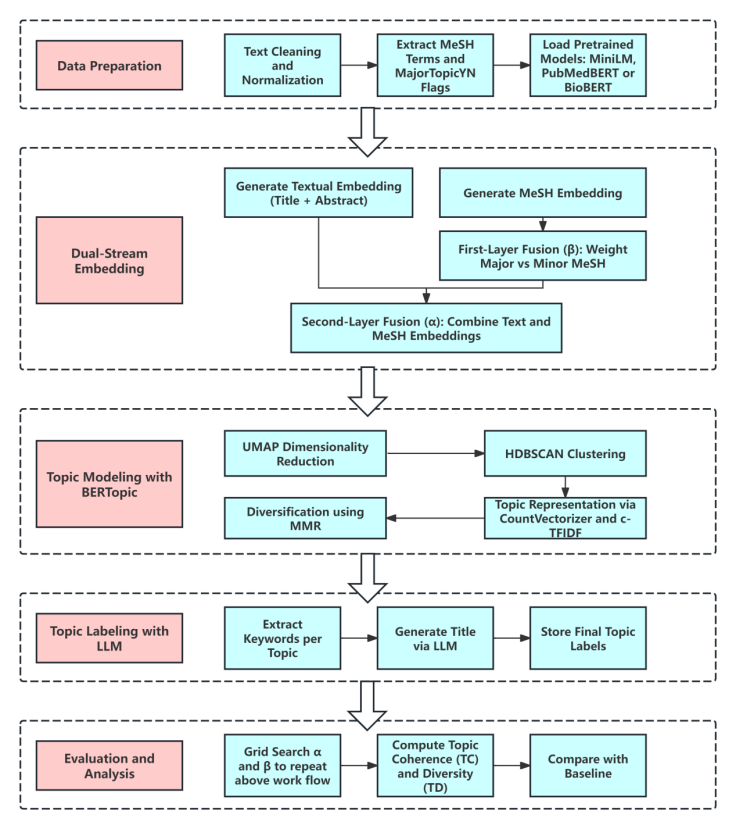
\includegraphics[width=8cm]{./fig/figure1.png}
\caption{System workflow of the proposed dual-stream topic modelling framework.}
\label{fig1}
\end{figure}

In the data preparation stage, article titles, abstracts, and MeSH descriptors are extracted from PubMed records. Each MeSH term is associated with a binary MajorTopicYN flag that indicates whether the term represents a major or minor topic. Pretrained transformer models---including MiniLM, PubMedBERT, and BioBERT---are loaded for downstream embedding generation.
In the dual-stream embedding stage, two parallel embedding vectors are computed: one for unstructured biomedical text (titles and abstracts) and the other for structured MeSH descriptors. The MeSH stream is processed through a first-layer fusion mechanism, which applies a weighting scheme controlled by parameter $\beta$ to emphasize major MeSH terms over minor ones. The resulting weighted MeSH embedding is then combined with textual embedding via a second-layer fusion mechanism governed by parameter $\alpha$, which balances the contributions of textual and MeSH streams to form the final document representation.
In the topic modelling stage, the fused embeddings are fed into the BERTopic pipeline. Dimensionality reduction is performed via UMAP, followed by clustering via HDBSCAN. Topic representations are generated via CountVectorizer and class-based TF-IDF (c-TF-IDF) and are further refined via maximal marginal relevance (MMR) to improve interpretability by promoting keyword diversity.
In the topic labelling stage, the top-ranked keywords from each topic are extracted and used to prompt a large language model (LLM) to generate concise, human-readable topic titles. This step improves accessibility for users without domain expertise and supports downstream applications such as thematic dashboards and visualizations.
In the evaluation and analysis stage, a grid search is conducted over the $\alpha$ and $\beta$ values to explore the parameter space. For each configuration, topic coherence (TC) and topic diversity (TD) are computed to assess the semantic quality of the generated topics. These results are compared against those of single-stream and ablation baselines to validate the performance improvements introduced by the dual-layer fusion mechanism.

\subsection{Dataset}
The dataset used in this study comprises 3,000 biomedical article records retrieved from the PubMed database. Each record contains the article title, abstract, publication year, PubMed ID (PMID), and associated MeSH (Medical Subject Headings) terms. To ensure comparability with existing methods and enable a controlled baseline comparison, we adopted the exact dataset and preprocessing methodology used in the study ``Depression, anxiety, and burnout in academia: topic modeling of PubMed abstracts''\cite{lezhnina_depression_2023}. This ensures that any observed differences in topic quality or interpretability are attributable to the modelling framework rather than variations in data sourcing or processing.
The PubMed records are structured according to the MEDLINE format, which includes metadata such as titles, abstracts, publication dates, and manually assigned Medical Subject Headings (MeSHs). Each MeSH term is accompanied by a MajorTopicYN flag, indicating whether the term represents a primary subject focus (MajorTopicYN=Y) or a secondary/supporting concept (MajorTopicYN=N). In this study, we utilize this binary distinction to inform the $\beta$-weighted fusion of MeSH embeddings, thereby emphasizing core medical topics during the integration process.

\subsection{Data Preprocessing}
Minimal preprocessing was required due to the design of the embedding framework. Specifically, we employed models from the Sentence Transformers library, which utilize pretrained transformer-based encoders that are robust to raw, unprocessed text input\cite{reimers_sentence-bert_2019}. Unlike traditional bag-of-words topic models, which often require lower casing, lemmatization, stopword removal, or token filtering, transformer-based sentence embeddings inherently capture contextual semantics without relying on such preprocessing steps. This aligns with findings from prior studies that show that modern sentence embedding models can operate effectively on unaltered text, preserving more nuanced linguistic and biomedical structures\cite{wang_graph-embedded_2022}. Specifically, the subword (WordPiece/BPE) tokenization used by these encoders already decomposes rare or morphologically complex biomedical terms into known sub-units, so lemmatization and aggressive token filtering are unnecessary; conversely, stopword removal and lowercasing would discard casing and function-word cues that the transformer's contextual attention exploits, and could therefore degrade rather than improve the embeddings. As such, our pipeline did not apply additional text normalization procedures beyond basic format verification.

The preprocessing workflow transforms raw PubMed records into structured document representations suitable for the dual-stream embedding framework. Each record undergoes systematic extraction of core components (title, abstract, MeSH terms, PMID, and publication year), followed by format verification and MeSH metadata structuring. Critically, the MajorTopicYN flag associated with each MeSH term is preserved during this stage, enabling the subsequent parameterized fusion mechanism to distinguish between major and minor topics. The complete preprocessing procedure is formalized in Algorithm~\ref{alg:preprocessing}.

\begin{algorithm*}[t]
\caption{Biomedical Document Preprocessing for Transformer-Based Embeddings}
\label{alg:preprocessing}
\begin{algorithmic}[1]
\Require Raw PubMed records $R = \{r_1, r_2, \ldots, r_n\}$
\Ensure Preprocessed documents $D = \{d_1, d_2, \ldots, d_n\}$ with verified MeSH metadata

\State Initialize empty document collection $D \gets \emptyset$

\For{each record $r_i \in R$}
    \State \textbf{// Extract core components}
    \State $\text{title} \gets \text{Extract\_Title}(r_i)$; $\text{abstract} \gets \text{Extract\_Abstract}(r_i)$; $\text{mesh\_terms} \gets \text{Extract\_MeSH\_Terms}(r_i)$
    \State $\text{pmid} \gets \text{Extract\_PMID}(r_i)$; $\text{pub\_year} \gets \text{Extract\_Publication\_Year}(r_i)$

    \State \textbf{// Format verification}
    \State $\text{title} \gets \text{Verify\_Format}(\text{title})$; $\text{abstract} \gets \text{Verify\_Format}(\text{abstract})$

    \State \textbf{// Process MeSH descriptors with major/minor flags}
    \State $\text{mesh\_structured} \gets \emptyset$
    \For{each $\text{term} \in \text{mesh\_terms}$}
        \State $\text{descriptor} \gets \text{term.descriptor\_name}$; $\text{major\_flag} \gets \text{term.major\_topic\_yn}$
        \State $\text{mesh\_structured} \gets \text{mesh\_structured} \cup \{(\text{descriptor}, \text{major\_flag})\}$
    \EndFor

    \State \textbf{// Construct document representation and create object}
    \State $\text{full\_text} \gets \text{Concatenate}(\text{title}, \text{abstract}, \text{mesh\_terms})$
    \State $d_i.\text{pmid} \gets \text{pmid}$; $d_i.\text{title} \gets \text{title}$; $d_i.\text{abstract} \gets \text{abstract}$
    \State $d_i.\text{mesh\_terms} \gets \text{mesh\_structured}$; $d_i.\text{full\_text} \gets \text{full\_text}$; $d_i.\text{pub\_year} \gets \text{pub\_year}$

    \State \textbf{// Validate and add to collection}
    \If{$\text{Has\_Required\_Fields}(d_i)$}
        \State $D \gets D \cup \{d_i\}$
    \EndIf
\EndFor

\State \Return $D$
\end{algorithmic}
\end{algorithm*}

The preprocessing algorithm employs three helper functions to ensure data quality: (i) \textit{Verify\_Format} performs minimal text cleaning by removing null characters and stripping leading/trailing whitespace while preserving the original text structure; (ii) \textit{Has\_Required\_Fields} validates document completeness by ensuring that title, abstract, and MeSH terms are all non-empty ($\text{document.title} \neq \emptyset \land \text{document.abstract} \neq \emptyset \land \text{document.mesh\_terms} \neq \emptyset$); and (iii) \textit{Concatenate} combines the title, abstract, and MeSH descriptors into a unified full-text representation using space separators.

\subsection{Dual-Stream Embedding Framework}
The proposed dual-stream embedding framework is designed to integrate both unstructured textual content and structured biomedical metadata through two parallel embedding channels: a textual stream and a MeSH stream.
In this study, both the embedding inputs and the BERTopic document inputs were derived strictly from the full-text combination (Title + Abstract + MeSH). We employed models from the Sentence Transformers library to generate sentence-level embeddings from this unified input. This choice is motivated by the relatively long and syntactically rich nature of biomedical abstracts, where sentence-level transformers have demonstrated strong performance in capturing contextual semantics and discourse-level coherence\cite{reimers_sentence-bert_2019}. Additionally, sentence transformer models offer superior robustness in downstream integration scenarios, making them well suited for incorporation into real-world biomedical search systems.
For the MeSH stream, which represents the structured, domain-specific descriptors associated with each article, we explored two types of embeddings:
\begin{itemize}
    \item A Sentence Transformer model pretrained on biomedical corpora (NeuML/pubmedbert-base embedding)
    \item The original BioBERT model (dmis-lab/biobert-v1.1) with mean pooling was applied.
\end{itemize}
We compare which embedding strategy better captures the semantics of MeSH terms, which are typically composed of concise biomedical phrases or terminology.

\subsection{Parameterized Weighted Fusion Mechanism}
To effectively integrate both unstructured textual content and structured biomedical metadata,
a two-layer parameterized weighted fusion mechanism was developed.
This design governs the combination of
(i) sentence-level embeddings derived from article titles and abstracts (the text stream) and
(ii) embeddings generated from Medical Subject Headings (MeSH) descriptors (the MeSH stream).

Two scalar parameters control the fusion process:
\begin{itemize}
    \item \textbf{Text--MeSH fusion weight ($\boldsymbol{\alpha}$)}: adjusts the relative importance of text embeddings.
    \item \textbf{Major--Minor MeSH weighting parameter ($\boldsymbol{\beta}$)}: adjusts the relative per-term weight assigned to major versus minor MeSH terms based on the \textit{MajorTopicYN} flag.
\end{itemize}

Both $\boldsymbol{\alpha}$ and $\boldsymbol{\beta}$ are tunable within the range [0.05, 0.95] with a step size of 0.05.

\noindent\textbf{First-layer fusion: intra-MeSH term weighting ($\boldsymbol{\beta}$).}
Each article's MeSH terms are first categorized as either major or minor using the \textit{MajorTopicYN} flag.
Each term is encoded using a biomedical transformer model (e.g., BioBERT or PubMedBERT) and assigned a weight based on its importance:

\begin{itemize}
    \item \textbf{Major topic:} weight $= \boldsymbol{\beta}$
    \item \textbf{Minor topic:} weight $= 1 - \boldsymbol{\beta}$
\end{itemize}

The weights are then normalized, and the weighted average embedding for MeSH terms is computed as follows:
\begin{equation}
\text{MeSH\_Embedding} = \sum_i (w_i \times e_i)
\label{eq:mesh_embedding}
\end{equation}

where $e_i$ denotes the embedding of the $i$-th MeSH term and $w_i$ is its normalized weight.
This vector captures structured biomedical knowledge with an emphasis on core medical concepts.

\noindent\textbf{Second-layer fusion: text--MeSH stream integration ($\boldsymbol{\alpha}$).}
The final document-level embedding is constructed by blending the MeSH embedding and the text embedding through the parameter $\boldsymbol{\alpha}$, as follows:
\begin{equation}
\boldsymbol{e}_{\text{combined}} = \boldsymbol{\alpha} \cdot \boldsymbol{e}_{\text{text}} + (1 - \boldsymbol{\alpha}) \cdot \boldsymbol{e}_{\text{MeSH}}
\label{eq:combined_embedding}
\end{equation}
where $\boldsymbol{e}_{\text{combined}}$ denotes the final combined embedding, $\boldsymbol{e}_{\text{text}}$ is the text embedding, and $\boldsymbol{e}_{\text{MeSH}}$ is the weighted MeSH embedding from Equation~(\ref{eq:mesh_embedding}).

If an article does not contain MeSH terms, the text embedding alone is used.
All articles in the dataset utilized in this study contain MeSH descriptors.

\noindent\textbf{Implementation.}
The fusion mechanism was implemented as follows:
\begin{enumerate}[leftmargin=*,label=\arabic*.]
    \item Extract MeSH descriptors and mark each as major or minor.
    \item Encode each descriptor with a pretrained biomedical encoder to obtain embeddings.
    \item Assign weights $\beta$ (major) and $(1-\beta)$ (minor), normalize the weights, and compute the weighted sum of MeSH embeddings.
    \item Compute the final embedding as $\alpha\cdot\text{text\_embedding} + (1-\alpha)\cdot\text{mesh\_embedding}$ when MeSH exists; otherwise use the \text{text\_embedding}.
\end{enumerate}

The complete fusion logic is formalized in Algorithm~\ref{alg:mesh_fusion}.

\begin{algorithm}[H]
\caption{Text--MeSH Fusion with Major/Minor Weights}
\label{alg:mesh_fusion}
\begin{algorithmic}[1]
\Require Text embedding $\boldsymbol{t}$; MeSH descriptors $\{\boldsymbol{e}_1,\ldots,\boldsymbol{e}_n\}$ with major/minor flags $\{m_i\}$; parameters $\alpha,\beta$
\Ensure Combined embedding $\boldsymbol{c}$

\For{$i = 1$ to $n$}
    \State $w_i \gets \beta$ \textbf{if} $m_i = \texttt{True}$ \textbf{else} $1-\beta$
\EndFor

\State $\boldsymbol{w} \gets \mathrm{Normalize}([w_1,\ldots,w_n])$
\State $\boldsymbol{m} \gets \sum_{i=1}^{n} (w_i \cdot \boldsymbol{e}_i)$

\If{$\mathrm{has\_MeSH}(E) = \texttt{True}$}
    \State $\boldsymbol{c} \gets \alpha \cdot \boldsymbol{t} + (1-\alpha) \cdot \boldsymbol{m}$
\Else
    \State $\boldsymbol{c} \gets \boldsymbol{t}$
\EndIf

\State \Return $\boldsymbol{c}$
\end{algorithmic}
\end{algorithm}

\subsection{Design Rationale and Benefits}
This dual-stream embedding framework offers several advantages:
\begin{enumerate}[leftmargin=*,label=\arabic*)]
    \item \textbf{Semantic complementarity:} The method integrates contextual semantics from free text with structured domain knowledge from curated vocabularies, providing a more comprehensive representation of document content.

    \item \textbf{Fine-grained control:} Adjustable parameters ($\alpha$ and $\beta$) enable the framework to adapt to varying corpus characteristics and information retrieval objectives, allowing task-specific optimization.

    \item \textbf{Interpretability:} The explicit separation and weighting of text and MeSH components enhance model transparency, facilitating understanding of the retrieval mechanism and promoting user trust.
\end{enumerate}

It is worth clarifying that, in the current framework, MeSH descriptors are deliberately treated as independent terms: each descriptor is encoded individually and the descriptors are aggregated by a weighted average, without explicitly modelling the MeSH tree hierarchy, synonym (entry-term) mappings, or subheading qualifiers. This is a considered design choice rather than an oversight. First, the contextual encoders used here (PubMedBERT, BioBERT) are pretrained on large biomedical corpora and therefore already capture a substantial degree of semantic relatedness between hierarchically or synonymously linked descriptors, so part of the structural signal is recovered implicitly through the embedding space. Second, relying only on the descriptor strings and the binary \textit{MajorTopicYN} flag keeps the method dependent solely on fields present in every MEDLINE record, making it broadly applicable and avoiding a dependence on the full MeSH ontology being available and correctly parsed. Third, and most importantly, this minimal formulation isolates the contribution of the dual-stream architecture itself from the orthogonal question of how richly the MeSH structure is exploited, yielding a clean and controlled comparison against the baseline. We none the less recognize that the MeSH hierarchy, qualifiers, and synonym relations encode additional expert knowledge that a simple average cannot represent; exploiting them explicitly is a promising direction that we return to in Section~5.

\subsection{Topic Modelling Pipeline}

\begin{figure}[H]
\centering
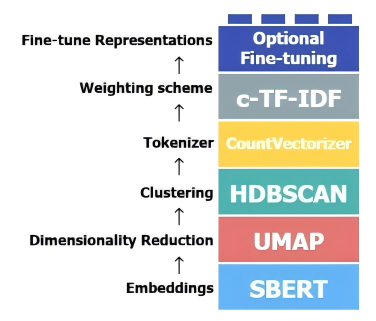
\includegraphics[width=8cm]{./fig/bertopic_pipeline.png}
\caption{Modular architecture of the BERTopic pipeline.}
\label{fig:bertopic_pipeline}
\end{figure}

To model latent thematic structures in the biomedical literature, we adopted the BERTopic framework~\cite{grootendorst_bertopic_2022}, a modular and extensible pipeline that integrates state-of-the-art sentence embeddings with clustering and keyword extraction. BERTopic is particularly well suited for biomedical domain applications because of its ability to generate interpretable topics from high-dimensional contextual embeddings via a structured and visually interpretable workflow (see \textbf{Fig.~\ref{fig:bertopic_pipeline}}).

To ensure rigorous and fair experimental comparison, we strictly replicated the full modelling pipeline and hyperparameter configurations from the target baseline study~\cite{lezhnina_depression_2023}. This ensures that all observed differences in topic quality stem solely from our proposed embedding strategies rather than from downstream modelling variations.

The BERTopic pipeline, illustrated in \textbf{Fig.~\ref{fig:bertopic_pipeline}}, consists of the following key components:

\begin{itemize}[leftmargin=*,itemsep=2pt]
    \item Sentence-level embeddings were generated via our dual-stream embedding framework and served as the input to the topic modelling pipeline.

    \item Dimensionality reduction was performed via UMAP, with the parameters set to \texttt{n\_neighbors}$=15$, \texttt{n\_components}$=5$, and \texttt{min\_dist}$=0.0$. These are the standard BERTopic defaults: \texttt{n\_neighbors}$=15$ balances the preservation of local and global structure, \texttt{min\_dist}$=0.0$ produces tightly packed embeddings that favour downstream density-based clustering, and \texttt{n\_components}$=5$ retains sufficient variance while mitigating the curse of dimensionality for HDBSCAN.

    \item Document clustering was conducted via HDBSCAN, which is configured with \texttt{min\_cluster\_size}$=30$ and \texttt{min\_samples}$=10$, enabling the discovery of semantically coherent clusters without predefining the number of topics. \texttt{min\_cluster\_size}$=30$ was adopted from the baseline study to ensure a directly comparable number of topics on the 3{,}000-document corpus---large enough to suppress spurious micro-clusters yet small enough to retain fine-grained themes---and \texttt{min\_samples}$=10$ provides a conservative noise threshold that limits over-fragmentation.

    \item Tokenization and keyword extraction rely on CountVectorizer and the ClassTfidfTransformer (c-TF-IDF) to compute discriminative topic representations.

    \item To promote topic interpretability and reduce keyword redundancy, maximal marginal relevance (MMR) was applied with a diversity parameter of 0.2.

    \item No modifications were made to any of the above components, preserving complete alignment with the baseline.
\end{itemize}

This strict adherence to the baseline modelling setup isolates the impact of the dual-stream embedding framework under equivalent downstream conditions.

\subsection{Evaluation Metrics Overview}
To evaluate topic modelling quality, we adopted two widely used metrics: topic coherence (TC) and topic diversity (TD). TC quantifies the semantic consistency of the top-ranked words within a topic, while TD measures the distinctiveness between topics by assessing vocabulary overlap. These metrics were chosen to ensure comparability with the baseline study~\cite{lezhnina_depression_2023} and are widely used in the neural topic modelling literature~\cite{dieng_topic_2020,mimno_optimizing_2011,roder_exploring_2015}.


\section{Experiment Design}
Experiments systematically explored the following:
\begin{enumerate}[leftmargin=*,label=\arabic*)]
    \item Four embedding model combinations (see \textbf{Table~\ref{tab:model_combinations}}).
    \item A comprehensive grid search of $\alpha$ and $\beta$ parameters across specified ranges.
\end{enumerate}

Preliminary experiments explored various text input strategies (Abstract, Text, Abmesh, and Full). However, all the final main experiments reported in this study exclusively adopted the full-text combination (Title~+~Abstract~+~MeSH) for both the embedding and BERTopic doc inputs, ensuring semantic alignment and eliminating input inconsistency.

\noindent\textbf{Computational cost and deployment considerations.}
The $\alpha$--$\beta$ grid search evaluates $19 \times 19 = 361$ parameter combinations per model over the range $[0.05, 0.95]$ with a step of $0.05$. Although the transformer encoders are the most expensive component of the pipeline, each document's text and MeSH-term embeddings are computed and cached only once; every grid cell then recomputes only the weighted fusion---an $\mathcal{O}(d)$ vector operation per document, where $d$ is the embedding dimension---followed by the BERTopic clustering stage (UMAP and HDBSCAN). The grid search is therefore dominated by lightweight clustering rather than by repeated neural encoding, and it is an offline, one-time tuning cost. At deployment time, once $\alpha$ and $\beta$ are fixed, embedding a new document requires only a single text encoding, a single MeSH encoding, and the $\mathcal{O}(d)$ fusion, adding negligible overhead over a standard single-stream BERTopic pipeline. The search is also embarrassingly parallel across grid cells, so wall-clock time scales inversely with the available compute.

\begin{table*}[!ht]
\caption{The four dual-stream embedding model combinations evaluated in this study, showing the transformer encoder assigned to the text stream and to the MeSH stream in each configuration.}
\label{tab:model_combinations}
\centering
\renewcommand{\arraystretch}{1.3}
\begin{tabular}{p{3.2cm}p{4.2cm}p{4cm}p{4.8cm}}
\hline
\textbf{Combinations Name} & \textbf{Text Stream Embedding Model} & \textbf{MeSH Stream Embedding Model} & \textbf{Description} \\
\hline
Dual PubMedBERT & NeuML/pubmedbert-base-embeddings & NeuML/pubmedbert-base-embeddings & Both streams use the biomedical PubMedBERT encoder. \\
\hline
Hybrid PubMedBERT-BioBERT & NeuML/pubmedbert-base-embeddings & dmis-lab/biobert-v1.1 & Hybrid model: PubMedBERT for the text stream and BioBERT for the MeSH stream. \\
\hline
Dual MiniLM (The Baseline's model) & all-MiniLM-L6-v2 & all-MiniLM-L6-v2 & Both streams use the general-purpose all-MiniLM-L6-v2 encoder adopted by the baseline study. \\
\hline
Dual BioBERT & dmis-lab/biobert-v1.1 & dmis-lab/biobert-v1.1 & Both streams use the biomedical BioBERT encoder. \\
\hline
\end{tabular}
\end{table*}

\subsection{Ablation Study Design}

We designed a controlled ablation study to isolate the contribution of architectural fusion from the raw information volume. Specifically, all ablation configurations use a single encoder model (all-MiniLM-L6-v2, same as the baseline) and avoid any fusion mechanism (no $\alpha$--$\beta$ weighting). Instead, multiple input sources are concatenated into a single textual stream, encoded via a single-stream embedding process. This allows us to evaluate whether comparable topic modelling performance can be achieved without structural fusion, given the same input information.

\subsection{Experimental Setup}

We evaluate four configurations, each constructed using different combinations of biomedical content (Title, Abstract, MeSH). In all the settings, the input components are concatenated into a single text sequence and embedded via the baseline model (all-MiniLM-L6-v2). This avoids architectural fusion or weight tuning, ensuring that any performance differences arise solely from the nature of the input data.

\begin{itemize}[leftmargin=*]
    \item \textbf{A1} -- Abstract only
    \item \textbf{A2} -- Title~+~Abstract
    \item \textbf{A3} -- Abstract~+~MeSH
    \item \textbf{A4} -- Title~+~Abstract~+~MeSH (Full input)
\end{itemize}

These configurations are then compared to two reference models:
\begin{enumerate}[leftmargin=*,label=\arabic*)]
    \item \textbf{Baseline:} Using only the abstract as the input, model with all-MiniLM-L6-v2, following prior studies.
    \item \textbf{Best dual-stream fusion model with the all-MiniLM-L6-v2 model:} The highest-performing configuration from the $\alpha$--$\beta$ tuned dual-stream experiments.
\end{enumerate}

The A1 (Abstract only) configuration replicates the baseline setting used in prior studies. For methodological rigor, we reran this configuration independently using our devices.

\subsection{Embedding Procedure}

For each configuration, the relevant text components are concatenated into a single string, which is then passed through the all-MiniLM-L6-v2 encoder to produce the document embedding. The resulting embeddings are directly used as inputs to the BERTopic pipeline (UMAP, HDBSCAN, c-TF-IDF), without modification or fusion. This ensures alignment with baseline processing while avoiding the additional complexity of multistream fusion.

\subsection{Evaluation Metrics}

To assess topic modelling performance, we adopted two widely used evaluation metrics: topic coherence (TC) and topic diversity (TD). These metrics were selected to ensure consistency with the baseline study~\cite{lezhnina_depression_2023}, thereby enabling direct comparison of topic modelling results.

\subsubsection{Topic Coherence (TC)}

Topic coherence (TC) quantifies the semantic consistency of a topic by evaluating the degree of co-occurrence among its top-ranked terms. Specifically, we use normalized pointwise mutual information (NPMI) over a reference corpus to compute coherence scores, following standard methodologies in the literature~\cite{mimno_optimizing_2011,roder_exploring_2015}.

\begin{equation}
TC = \frac{2}{N(N-1)} \sum_{i=1}^{N-1} \sum_{j=i+1}^{N} \text{NPMI}(w_i, w_j)
\label{eq:tc}
\end{equation}

To aid interpretability, we provide the following definitions of each variable in the evaluation metrics.

In Equation~(\ref{eq:tc}), the topic coherence (TC) score quantifies the semantic consistency among the top-ranked keywords of a given topic. Specifically:

\begin{itemize}
    \item where $N$ denotes the number of top terms considered per topic (e.g., $N = 10$).

    \item where $w_i$ and $w_j$ are the $i^{\text{th}}$ and $j^{\text{th}}$ words among the top $N$ words.

    \item where NPMI$(w_i, w_j)$ is the normalized pointwise mutual information between words $w_i$ and $w_j$, computed over a reference corpus (e.g., PubMed abstracts).
\end{itemize}

Equation~(\ref{eq:tc}) averages the pairwise NPMI scores across all unique word pairs in a topic, yielding a coherence score in the range $[-1, 1]$, where higher values indicate stronger semantic associations and better topic consistency.

\subsubsection{Topic Diversity (TD)}

Topic diversity (TD) assesses the distinctiveness between topics by computing the proportion of unique top-n words across all topics. Higher TD values indicate greater thematic breadth and reduced redundancy. This metric has been adopted in the neural topic modelling literature as a complementary measure to coherence~\cite{dieng_topic_2020}.

\begin{equation}
TD = \frac{\left|\bigcup_{k=1}^{K} \text{Top}_N(\text{Topic}_k)\right|}{K \times N}
\label{eq:td}
\end{equation}

In Equation~(\ref{eq:td}), the topic diversity (TD) score measures how distinct the topics are by evaluating vocabulary overlap:

\begin{itemize}
    \item $K$ is the total number of topics.

    \item where $\text{Top}_N(\text{Topic}_k)$ refers to the set of the top $N$ words in the $k^{\text{th}}$ topic.

    \item The numerator $\left|\bigcup_{k=1}^{K} \text{Top}_N(\text{Topic}_k)\right|$ counts the total number of unique terms across all the top $N$ word sets.

    \item The denominator $K \times N$ is the maximum possible number of distinct words if all topics are entirely disjoint.
\end{itemize}

The resulting TD value ranges from 0 to 1, where higher values indicate greater topic distinctiveness and reduced redundancy across topics.

These two metrics evaluate topic quality by capturing both intratopic semantic consistency and intertopic separation, which are essential for interpretability and downstream usability in biomedical literature applications.

\subsection{Comparison Protocol}
All the ablation results are evaluated via the same metrics as those used in the main study: topic coherence (TC), topic diversity (TD), and their sum (TC+TD). Each configuration is compared against

---the baseline model (Abstract only)

---the best-performing dual-stream framework model ($\alpha$--$\beta$ tuned, all-MiniLM-L6-v2 model).

This isolates the effect of information richness from structural innovation and validates whether multistream weighted integration is necessary for improved topic quality.

\subsection{Topic Label Enhancement with a Large Language Model (LLM)}

To improve the interpretability of the discovered topics, we integrated a postprocessing step using a large language model (LLM) via API calls. While BERTopic provides keyword-based topic representations, these keyword sets are often fragmented or require expert interpretation. To generate human-readable, semantically coherent topic titles suitable for academic use, we employed the Qwen-14B-Instruct model through the API.

Each topic's top keywords (obtained via BERTopic's c-TFIDF ranking) were used as input to a structured prompt. The prompt instructed the model to generate a concise and accurate English title that summarized the topic meaningfully, avoiding simple keyword repetition or direct translation. This approach aims to simulate expert-level summarization and provides titles that are suitable for inclusion in academic papers, visualizations, and topic-based exploration tools.

The generation pipeline included:

\begin{itemize}
    \item Cleaning and verifying the keyword format (ensuring a valid list of terms);
    \item Constructing a prompt template that contextualizes the generation task for the model;
    \item Iterative generation using qwen2.5-14b-instruct-1 m with a controlled decoding configuration (temperature=0.3, top\_p=0.95);
    \item The output is stored in the experimental result table alongside the raw keyword representations.
\end{itemize}

An example prompt used:

\begin{quote}
\textit{You are an expert in academic topic summarization. Please generate a concise, accurate, human-readable English title summarizing the following keywords: cancer, therapy, chemotherapy.}

\textit{Requirements:}
\begin{enumerate}
    \item \textit{Use one short sentence.}
    \item \textit{Focus on meaning, not literal translation or keyword listing.}
    \item \textit{The output should be English, be academic sounding, and be suitable for reports or visualizations.}
    \item \textit{Do not include quotes or numbering.}
\end{enumerate}

\textit{Please generate the topic title}
\end{quote}

This LLM-based topic labelling enhances downstream interpretability and provides a more intuitive interface for nonexpert users in literature exploration and clinical research.

\noindent\textbf{Reliability and alternative labelling strategies.}
Two points should be emphasized regarding the role and reliability of this component. First, LLM-generated titles are a presentation-layer enhancement only: the quantitative topic-quality metrics (TC and TD) are computed exclusively from the c-TF-IDF keyword distributions, so the labelling step does not influence any reported score and cannot inflate the comparison against the baseline. Second, the main reliability risk of LLM labelling is hallucination or over-generalization. We mitigate this by (i) constraining the prompt to summarize only the keywords supplied by BERTopic, without introducing external concepts, and (ii) using low-temperature decoding (temperature $=0.3$), which yields stable, near-deterministic titles across runs. Compared with alternative labelling strategies---raw c-TF-IDF keyword lists (the BERTopic default), KeyBERT-based keyphrase extraction, or selecting the most representative document title---the LLM approach produces fluent, self-contained titles that require no expert post-interpretation, at the cost of a dependence on an external model. Because the labelling layer is fully decoupled from the embedding and clustering stages, it can be replaced by any of these alternatives without affecting the dual-stream results.

\section{Results}

\subsection{Overall Experimental Outcomes}

Three of the four dual-stream embedding configurations outperformed the baseline, and the dual-stream fusion surpassed every single-stream ablation model built from the same inputs. Among all the configurations, the Dual PubMedBERT model achieved the highest overall topic modelling quality, with a topic coherence (TC) of 0.6172, a topic diversity (TD) of 0.7458, and a combined TC+TD score of 1.3443, representing a 7.3\% improvement over the baseline (TC+TD = 1.2530). These results demonstrate the effectiveness of integrating contextual textual embeddings with structured biomedical metadata under the proposed fusion mechanism.

To provide a more intuitive view of the parameter landscape, we visualized the $\alpha$--$\beta$ grid search results via three separate heatmaps:

\begin{figure}[htbp]
\centering
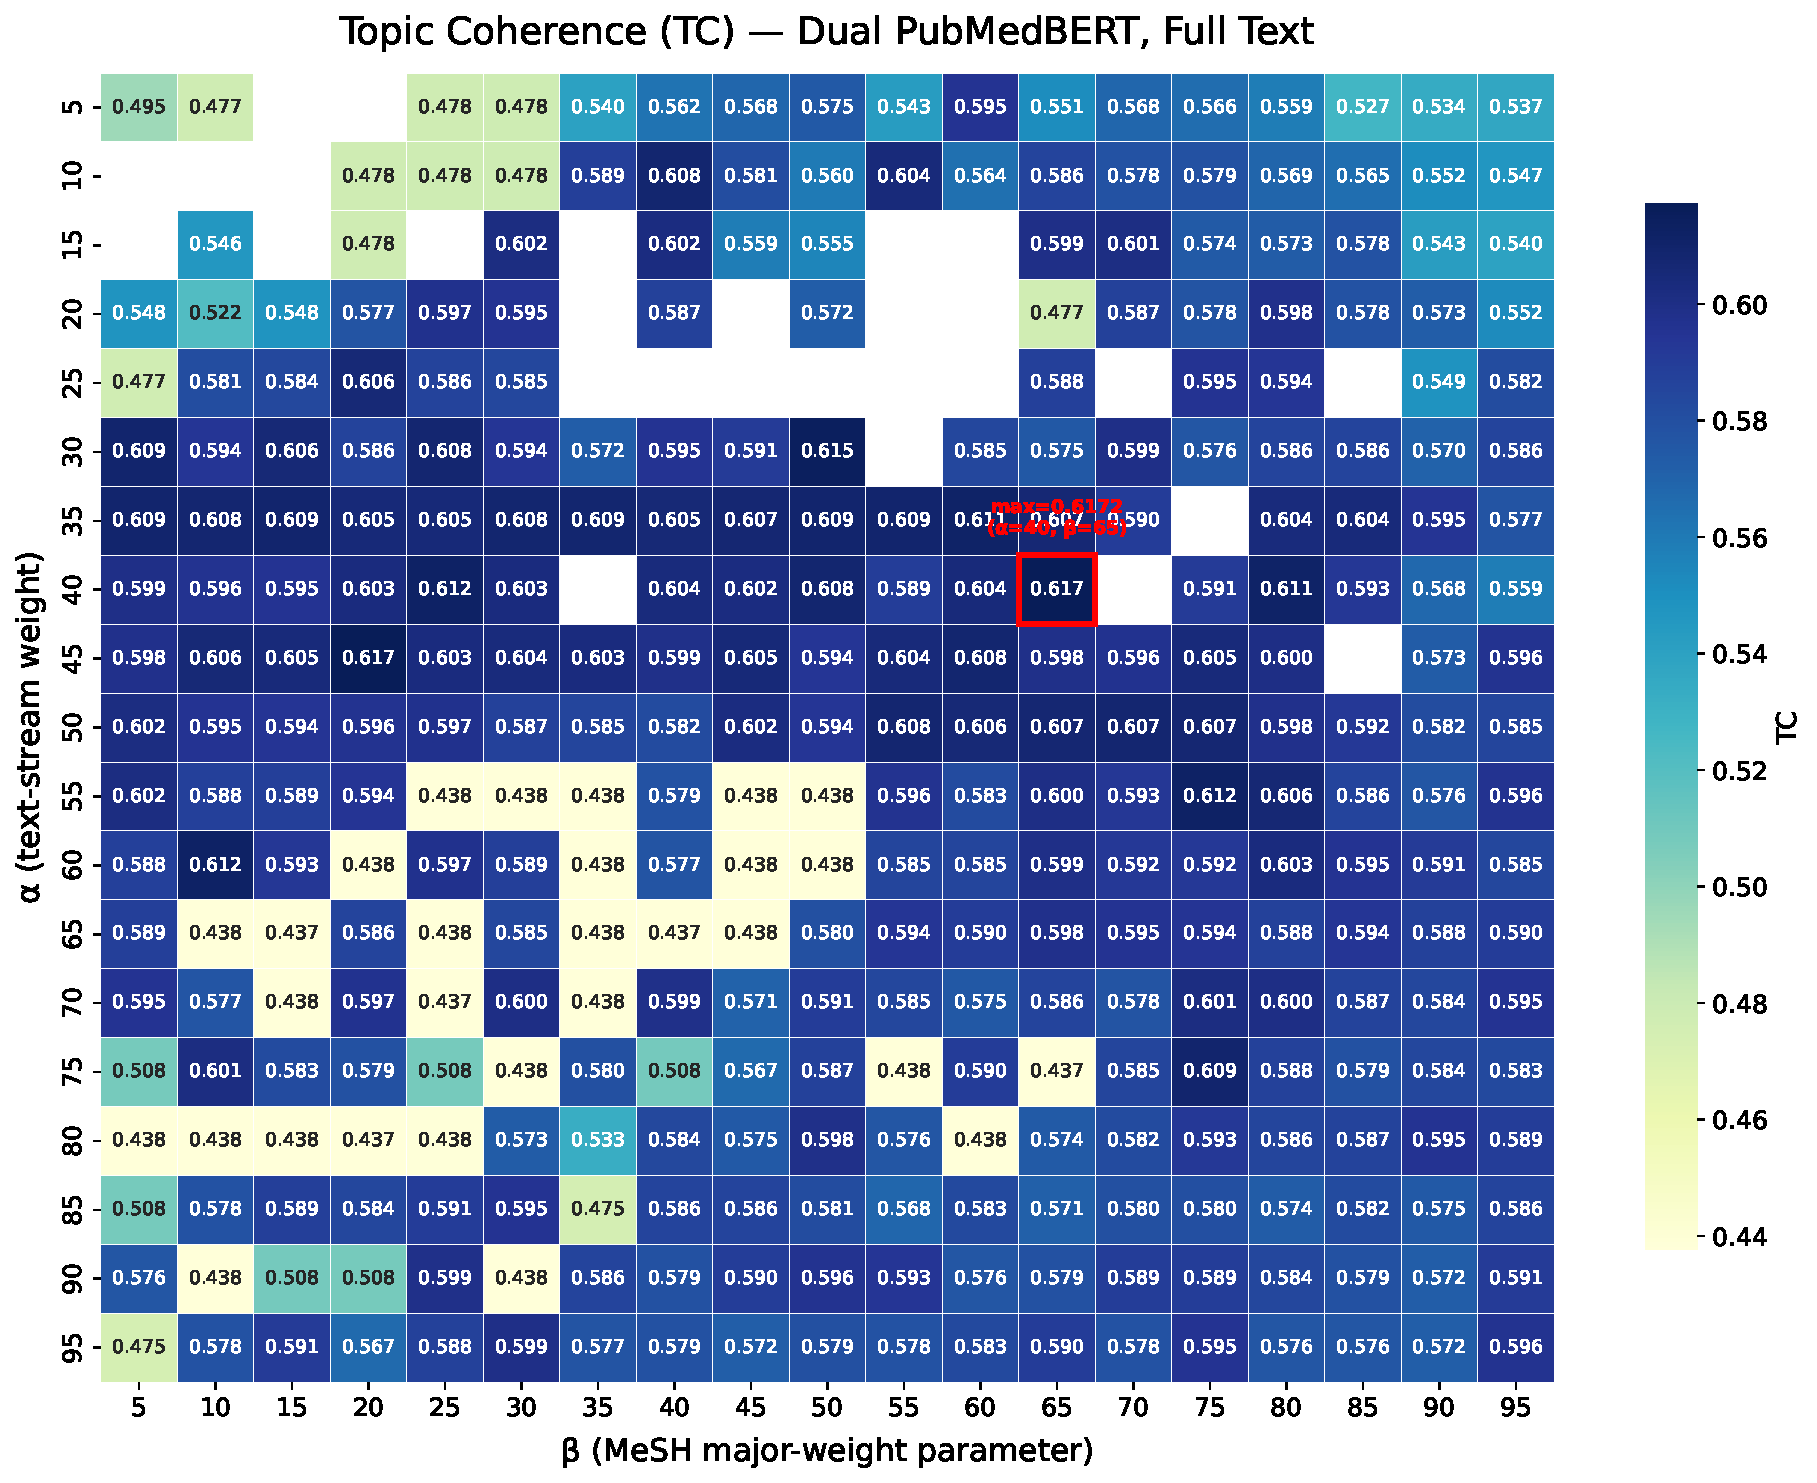
\includegraphics[width=8cm]{./fig/fig_tc_heatmap.pdf}
\caption{Heatmap of topic coherence (TC) scores across the $\alpha$--$\beta$ parameter grid under the Dual PubMedBERT configuration.}
\label{fig:tc_heatmap}
\end{figure}

\textbf{Figure~\ref{fig:tc_heatmap}} shows the distribution of topic coherence (TC) across different $\alpha$--$\beta$ combinations. The highest TC value of 0.6172 was achieved at $\alpha=0.40$ and $\beta=0.65$, indicating that emphasizing textual information alongside strongly weighted major MeSH terms leads to more semantically consistent topic clusters.

\begin{figure}[htbp]
\centering
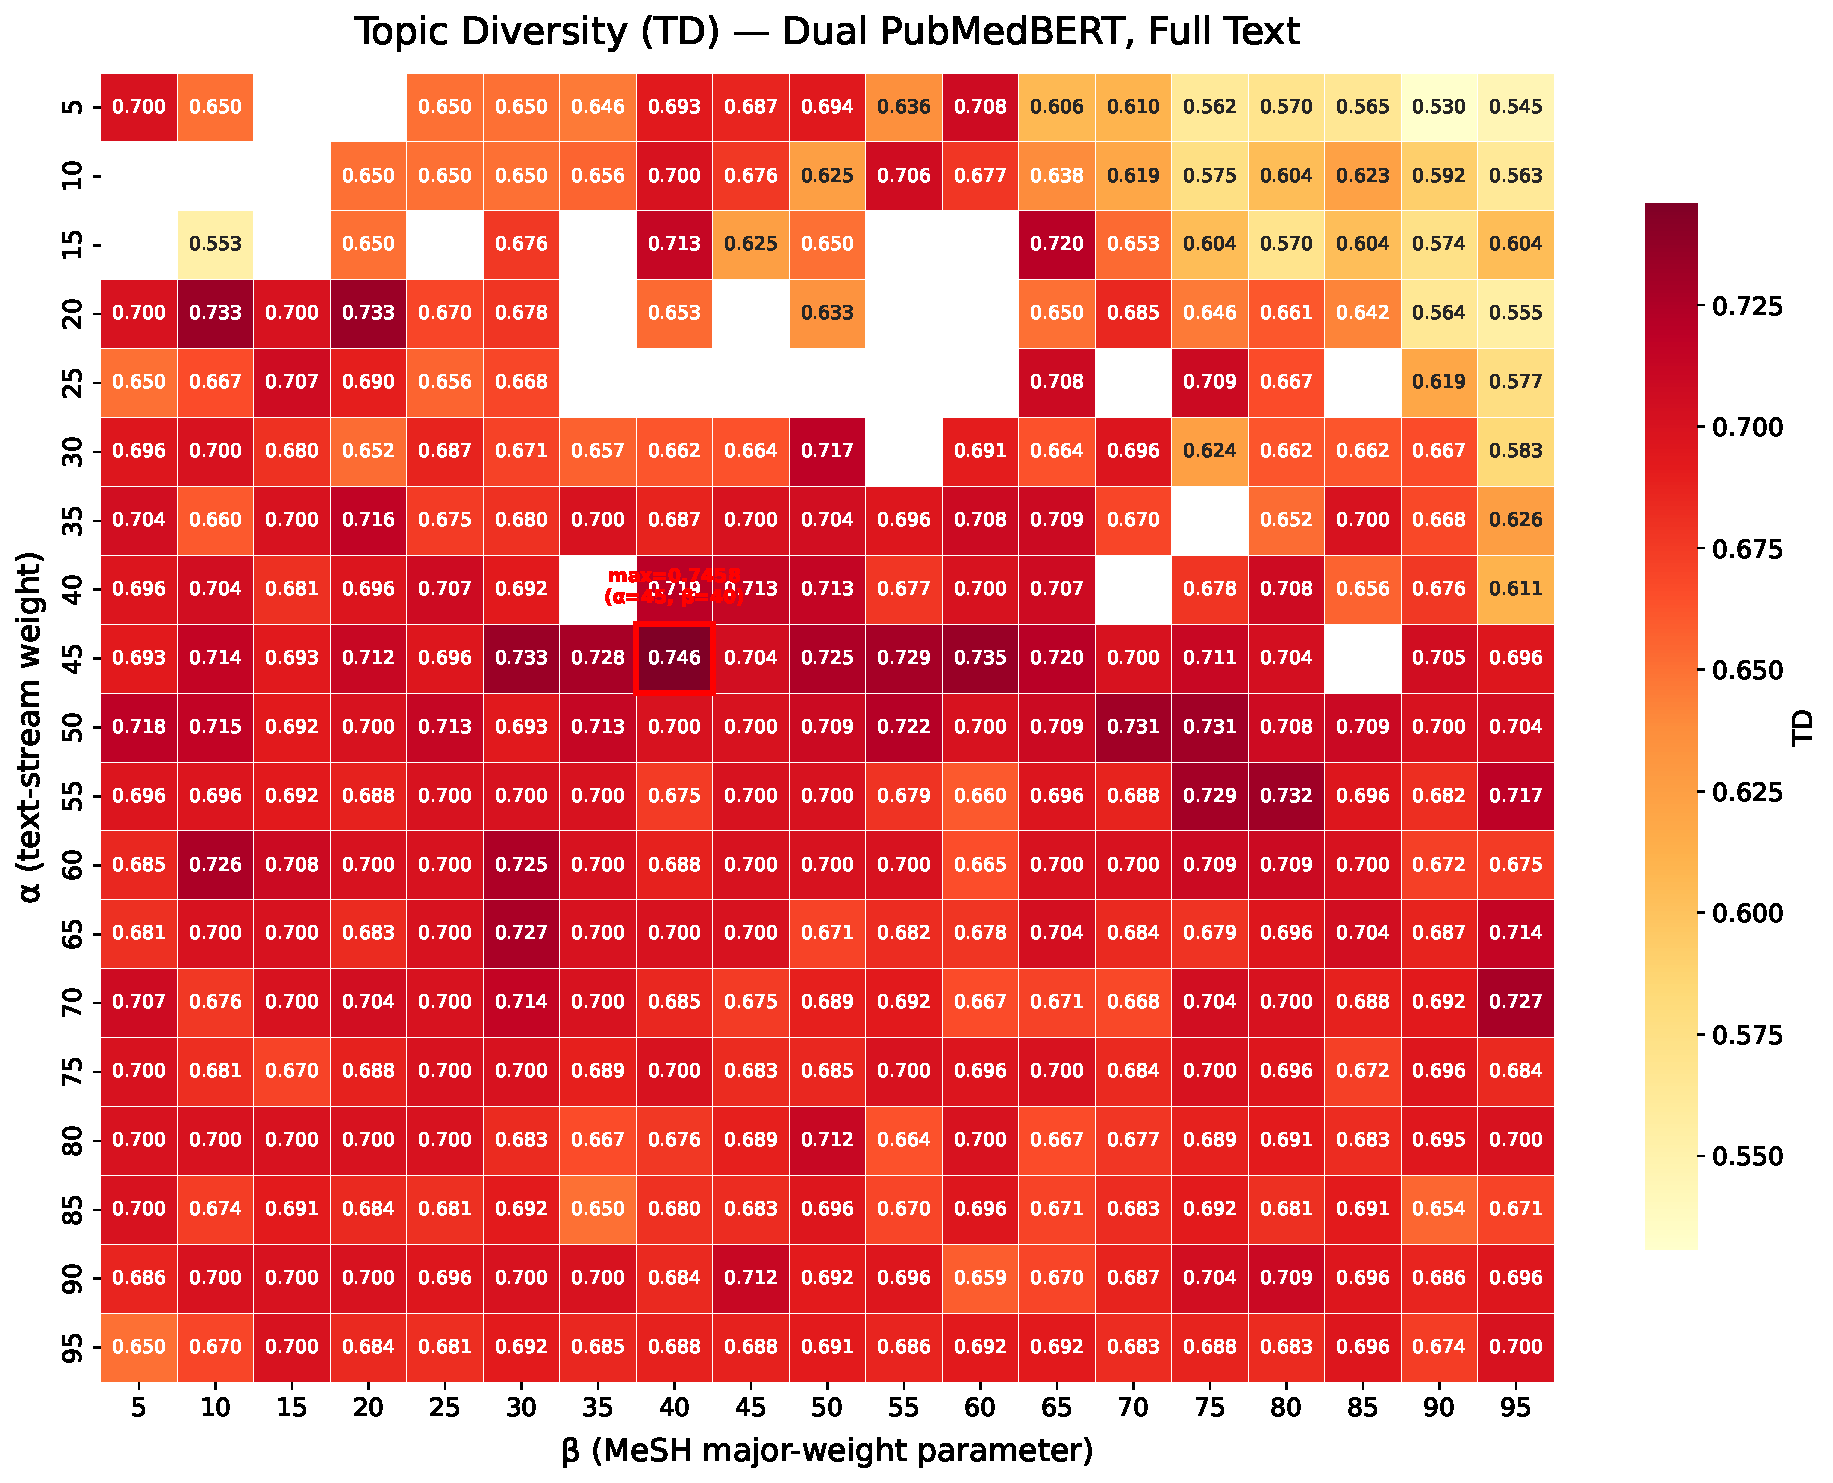
\includegraphics[width=8cm]{./fig/fig_td_heatmap.pdf}
\caption{Heatmap of topic diversity (TD) scores across the $\alpha$--$\beta$ parameter grid under the Dual PubMedBERT configuration.}
\label{fig:td_heatmap}
\end{figure}

\textbf{Figure~\ref{fig:td_heatmap}} illustrates the variation in topic diversity (TD). The highest TD score of 0.7458 occurred at $\alpha=0.45$ and $\beta=0.40$, suggesting that balanced weighting between textual and MeSH inputs fosters broader thematic coverage and reduced keyword overlap across topics.

\begin{figure}[htbp]
\centering
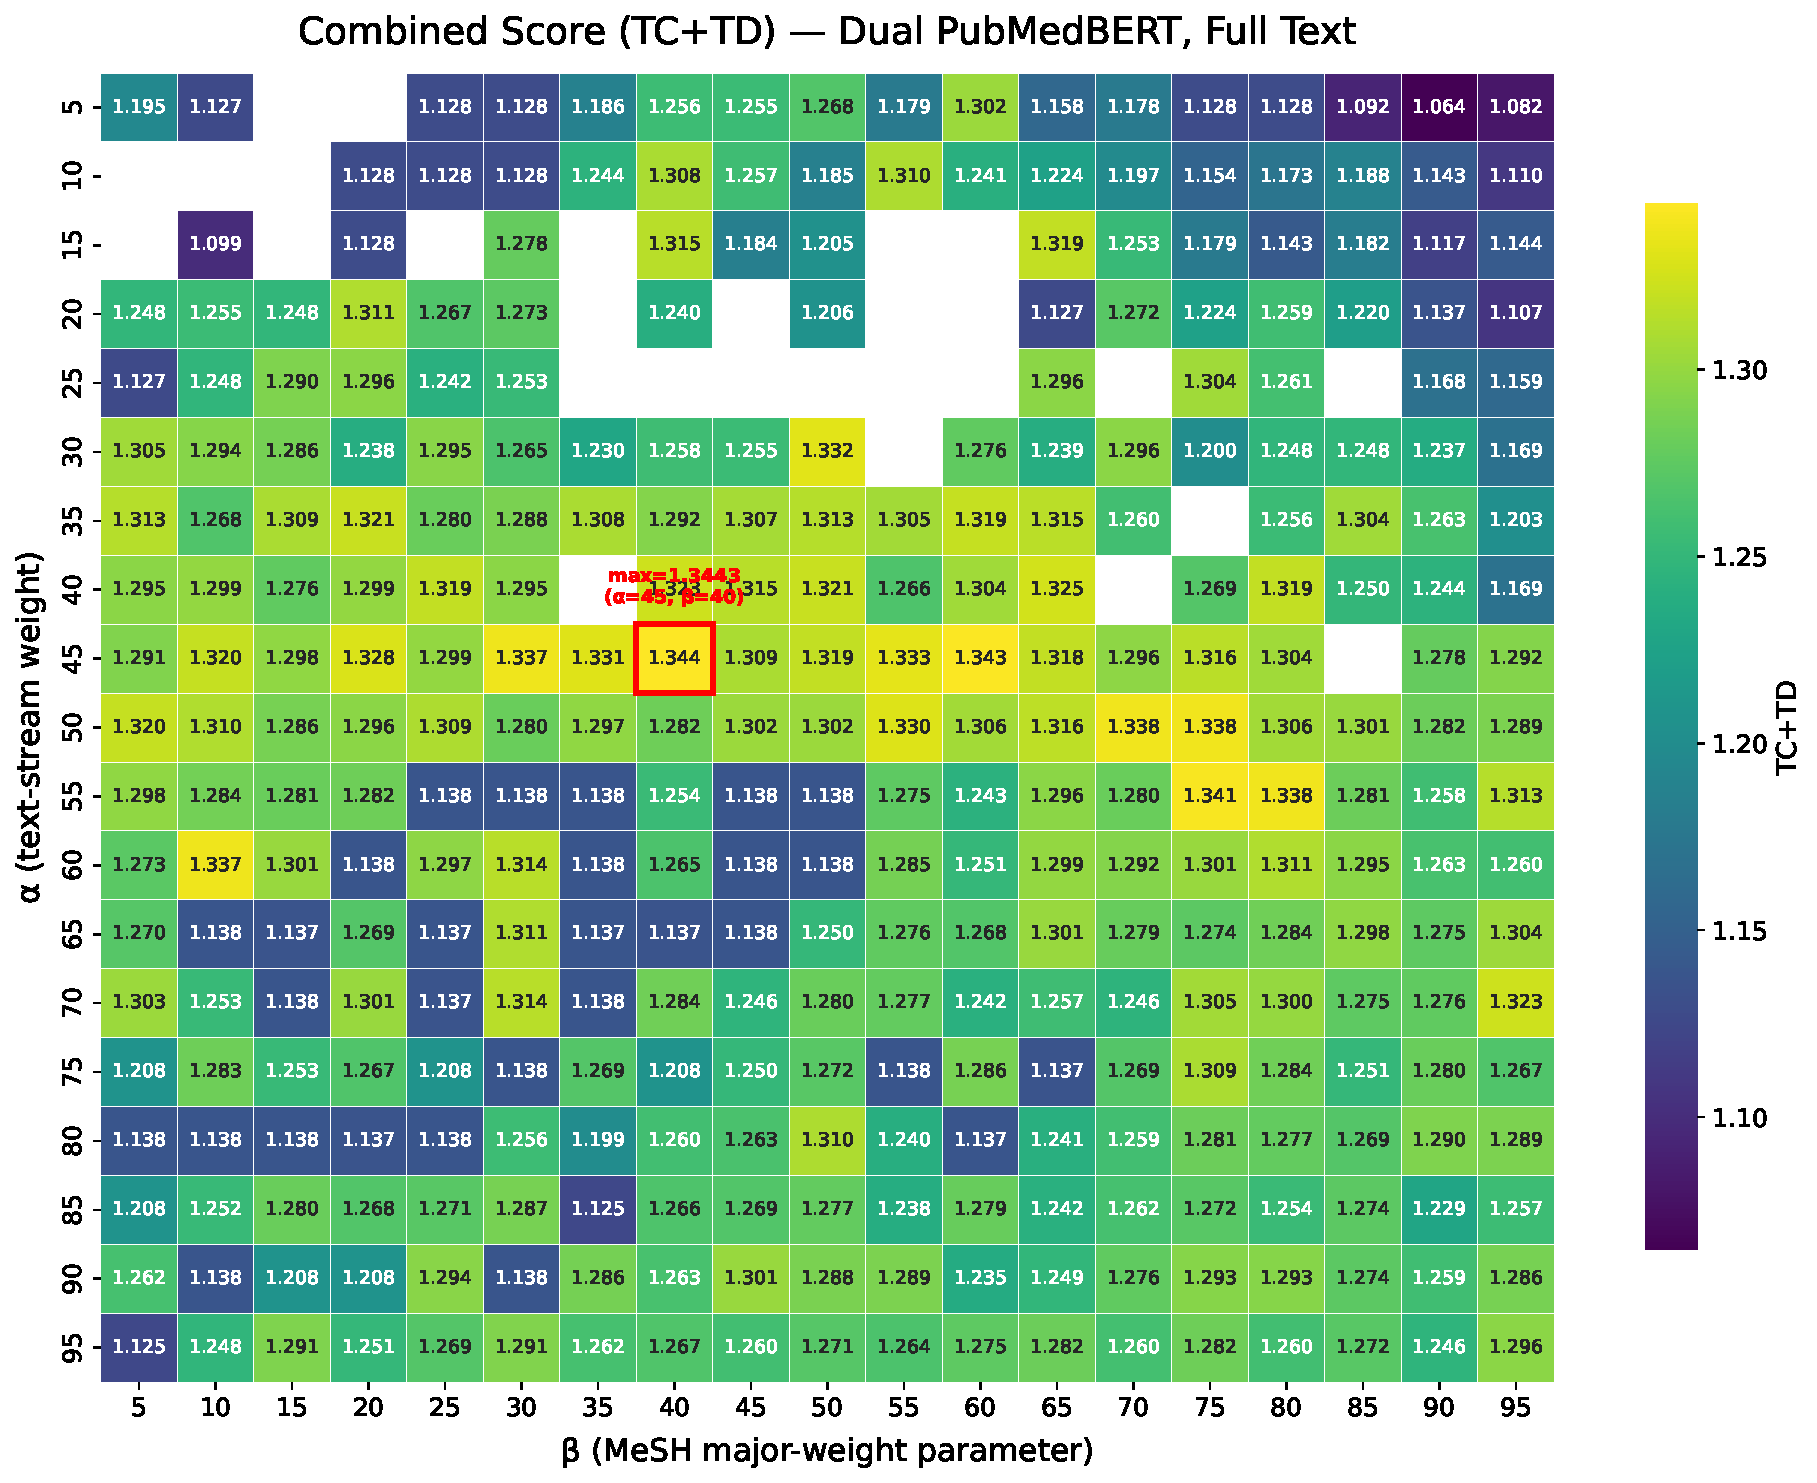
\includegraphics[width=8cm]{./fig/fig_combined_heatmap.pdf}
\caption{Heatmap of combined topic coherence and diversity scores across the $\alpha$--$\beta$ parameter grid under the Dual PubMedBERT configuration.}
\label{fig:combined_heatmap}
\end{figure}

\textbf{Figure~\ref{fig:combined_heatmap}} presents the combined TC+TD scores, reflecting the trade-off between intratopic coherence and intertopic diversity. The optimal joint performance (TC+TD = 1.3443) was also observed at $\alpha=0.45$ and $\beta=0.40$, confirming the robustness of this fusion configuration.

Blank regions in the heatmaps denote $\alpha$--$\beta$ combinations that produced an abnormally low number of clusters, typically fewer than five, making coherence and diversity scores unreliable. These were excluded from visualizations to ensure clarity and interpretability.

\subsection{Model-Specific Performance}

The dual-stream embedding topic modelling framework demonstrated significant improvements over baseline models across all evaluated metrics. The detailed performance of each model is summarized clearly in \textbf{Table~\ref{tab:model_performance}}.

\begin{table*}[t]
\centering
\caption{Best topic coherence (TC), topic diversity (TD), and combined TC+TD scores for each dual-stream model, with the corresponding optimal $(\alpha,\beta)$ parameters and the relative improvement over the single-stream baseline (TC+TD = 1.2530). Each metric column reports the best value attained over the $\alpha$--$\beta$ grid, which may occur at different parameter settings.}
\label{tab:model_performance}
\renewcommand{\arraystretch}{1.3}
\begin{tabular}{lcccc}
\hline
\textbf{Model} & \textbf{Best TC} & \textbf{Best TD} & \textbf{Best TC+TD} & \textbf{Improvement} \\
 & ($\alpha$, $\beta$) & ($\alpha$, $\beta$) & ($\alpha$, $\beta$) & \textbf{(vs. Baseline)} \\
\hline
\textbf{Dual PubMedBERT} & 0.6172 & 0.7458 & 1.3443 & +7.3\% \\
 & (0.40, 0.65) & (0.45, 0.40) & (0.45, 0.40) & \\
\hline
\textbf{Hybrid} & 0.6038 & 0.7333 & 1.3247 & +5.7\% \\
\textbf{PubMedBERT-BioBERT} & (0.15, 0.15) & (0.10, 0.25) & (0.30, 0.35) & \\
\hline
\textbf{Dual MiniLM} & 0.6076 & 0.7143 & 1.3005 & +3.8\% \\
\textbf{(The Baseline's model)} & (0.15, 0.20) & (0.10, 0.35) & (0.20, 0.35) & \\
\hline
\textbf{Dual BioBERT} & 0.5826 & 0.7000 & 1.2331 & -1.6\% \\
 & (0.45, 0.65) & (0.10, 0.15) & (0.45, 0.80) & \\
\hline
\textbf{Baseline} & 0.5360 & 0.7170 & 1.2530 & --- \\
\hline
\end{tabular}
\end{table*}

\begin{figure*}[!t]
\centering
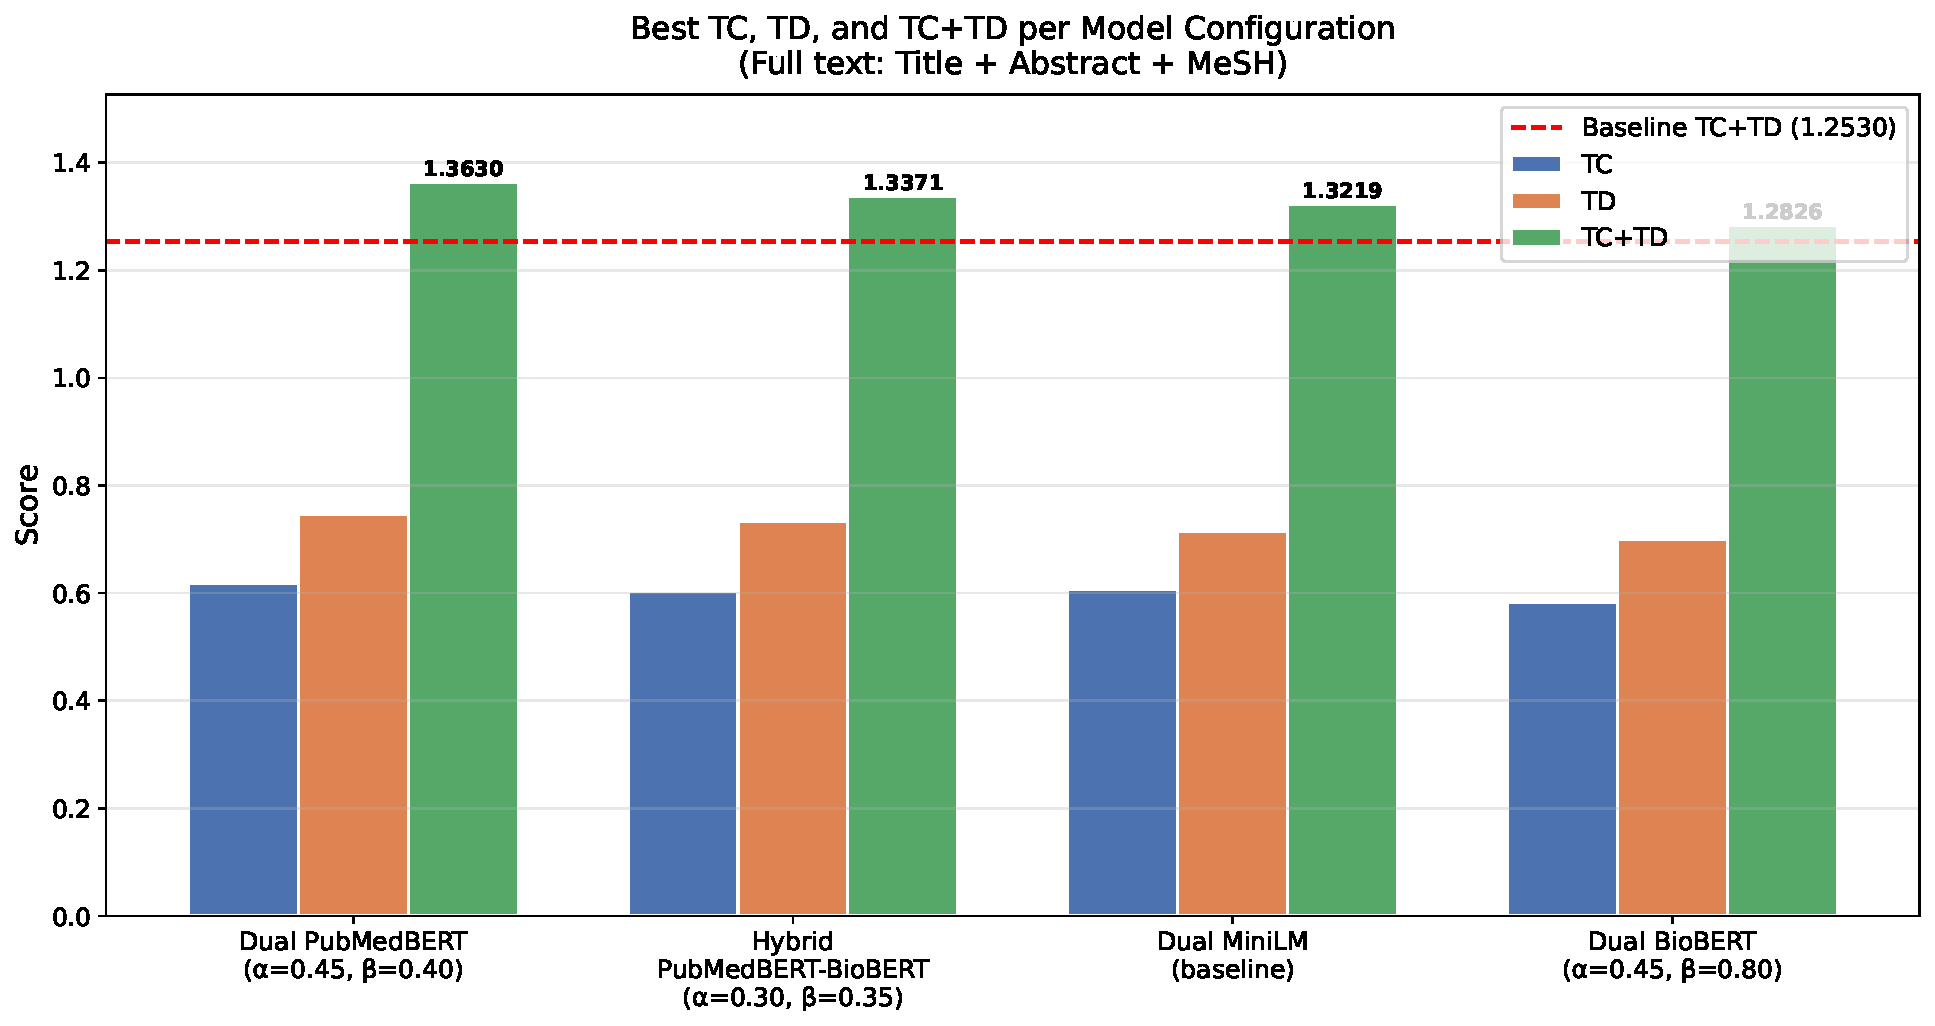
\includegraphics[width=12cm]{./fig/fig_model_comparison_bar.pdf}
\caption{Performance comparison of dual-stream model variants across TC, TD, and combined scores. Dual PubMedBERT achieves the highest combined score (TC+TD = 1.3443) with optimal parameters $\alpha=0.45$ and $\beta=0.40$. Data source: \textbf{Table~\ref{tab:model_performance}}.}
\label{fig:model_comparison}
\end{figure*}

\textbf{Table~\ref{tab:model_performance}} shows that, on the combined TC+TD metric, three of the four dual-stream configurations outperform the baseline, while Dual BioBERT falls slightly below it. Notably, the Dual PubMedBERT model achieved the highest performance, with clear improvements in both coherence and diversity over the baseline. As illustrated in \textbf{Fig.~\ref{fig:model_comparison}}, Dual PubMedBERT outperforms all other variants, achieving the highest combined score (TC+TD = 1.3443) at optimal parameters $\alpha=0.45$ and $\beta=0.40$. The hybrid configuration demonstrates competitive performance with TC+TD = 1.3247, while Dual BioBERT shows the lowest performance (TC+TD = 1.2331), even underperforming the baseline by $1.6\%$. This validates the importance of both model selection and proper hyperparameter tuning in the dual-stream framework.

To complement the aggregate metrics, we examined the statistical reliability of the coherence improvement at the topic level. Per-topic coherence ($c_v$) scores were computed for the optimal Dual PubMedBERT configuration ($\alpha=0.45$, $\beta=0.40$; 24 topics) and the single-stream baseline (all-MiniLM-L6-v2 on abstracts; 24 topics); these per-topic scores are obtained by topic-level decomposition and are not on the same scale as---and therefore not directly comparable to---the corpus-aggregate TC values reported in Table~\ref{tab:model_performance}. The dual-stream model attained a higher mean per-topic coherence (0.597 vs.\ 0.568); in a pairwise comparison, a randomly selected dual-stream topic exceeds a randomly selected baseline topic in coherence $56\%$ of the time. A one-sided Mann--Whitney~U test did not reach the conventional significance threshold ($p=0.25$). This is an expected consequence of the small number of topics ($n=24$) and the substantial inter-topic variance characteristic of topic models: topic-level inference is inherently low-powered, which is why topic-modelling studies---including the baseline study---conventionally evaluate performance through aggregate TC and TD rather than per-topic hypothesis testing. The consistent direction of the per-topic difference, combined with the improvement on both aggregate metrics at the optimal configuration, indicates that the gain reflects a systematic shift of the coherence distribution rather than a single high-scoring topic.

\subsection{Optimal Parameters and Robustness}

A comprehensive parameter analysis identified the optimal parameter ranges for the dual-stream fusion mechanism, which were concentrated around moderate values:

\begin{itemize}
    \item $\alpha$ (text vs. MeSH weighting): 0.15--0.45
    \item $\beta$ (major vs. minor MeSH weighting): 0.15--0.80
\end{itemize}

These parameter ranges indicate a balanced integration of textual content and structured biomedical knowledge, significantly enhancing both the coherence and diversity of discovered topics.

Compared with the baseline, the dual-stream models maintained reliable performance across a broad range of parameter settings, with the best configurations clustered in the moderate-value region of the $\alpha$--$\beta$ grid rather than at isolated extreme points, indicating that the framework is not unduly sensitive to fine parameter choices.

\subsection{Enhanced Interpretability Through Topic Labelling}

Applying the LLM-based topic-labelling procedure described above to the topics discovered by the best-performing configuration produced concise, human-readable titles in place of the raw keyword lists.

\begin{table*}[!t]
\centering
\caption{Representative examples of human-readable topic titles generated by the Qwen-14B LLM from BERTopic keyword sets, illustrating the interpretability gain over raw keyword lists.}
\label{tab:topic_labels}
\footnotesize
\begin{tabular}{c p{5.5cm} p{8cm}}
\hline
\textbf{Topic ID} & \textbf{Top Keywords} & \textbf{LLM-Generated Title} \\
\hline
\textbf{0} & students, nursing, medical, learning, clinical, student, education, anxiety, simulation, burnout & Addressing Anxiety and Burnout in Nursing Students through Clinical Simulation-Based Medical Education \\
\hline
\textbf{1} & health, mental, students, depression, prevalence, symptoms, data, factors, study, numerical & Numerical Study on the Prevalence of Depression Symptoms in Mental Health Among Students \\
\hline
\textbf{2} & covid19, pandemic, health, mental, students, anxiety, depression, pandemics, stress, study & Mental Health Impact of Anxiety and Depression on Students During the COVID-19 Pandemic \\
\hline
\textbf{3} & intervention, mindfulness, trial, treatment, group, stress, anxiety, control, therapy, randomized & Randomized Trial of Mindfulness Intervention for Stress and Anxiety in Treatment Groups \\
\hline
\textbf{4} & burnout, residents, residency, resident, training, medical, physicians, trainees, internship, survey & Burnout among medical residents and trainees during internship: a survey analysis \\
\hline
\end{tabular}
\end{table*}

\textbf{Table~\ref{tab:topic_labels}} illustrates five representative examples of LLM-generated titles. Each title corresponds to a unique topic and demonstrates how natural language summarization can bridge the gap between machine-generated keywords and human comprehension. The results show that LLM-based postprocessing significantly improves topic accessibility, reducing the cognitive effort needed to interpret and organize thematic outputs.

\subsection{Ablation Study Results}

To isolate the effectiveness of the proposed dual-stream fusion mechanism, we designed a set of ablation experiments using a fixed single-stream architecture without parameterized integration. Each configuration concatenated different combinations of textual and metadata inputs and encoded them via the baseline model (all-MiniLM-L6-v2) without applying any $\alpha$--$\beta$ fusion.

\begin{table*}[!t]
\centering
\caption{Ablation study results: topic coherence (TC), topic diversity (TD), and combined TC+TD scores for the single-stream input configurations A1--A4 (concatenated inputs, no $\alpha$--$\beta$ fusion), compared with the baseline and the full dual-stream model with parameterized fusion.}
\label{tab:ablation_results}
\begin{tabular}{cccccc}
\hline
\textbf{Experiment ID} & \textbf{Input Configuration} & \textbf{Input Components} & \textbf{TC} & \textbf{TD} & \textbf{TC+TD} \\
\hline
A1 & Abstract only & Abstract & 0.5428 & 0.7136 & 1.2564 \\
A2 & Text & Title + Abstract & 0.5355 & 0.6667 & 1.2022 \\
A3 & AbMeSH & Abstract + MeSH & 0.5274 & 0.6087 & 1.1361 \\
A4 & Full & Title + Abstract + MeSH & 0.5451 & 0.6174 & 1.1625 \\
\hline
Baseline & Abstract only & Abstract & 0.5360 & 0.7170 & 1.2530 \\
Dual-Stream & Full + $\alpha\beta$ Fusion & Title + Abstract + MeSH & 0.6047 & 0.6958 & 1.3005 \\
\hline
\end{tabular}
\end{table*}

\begin{figure*}[!t]
\centering
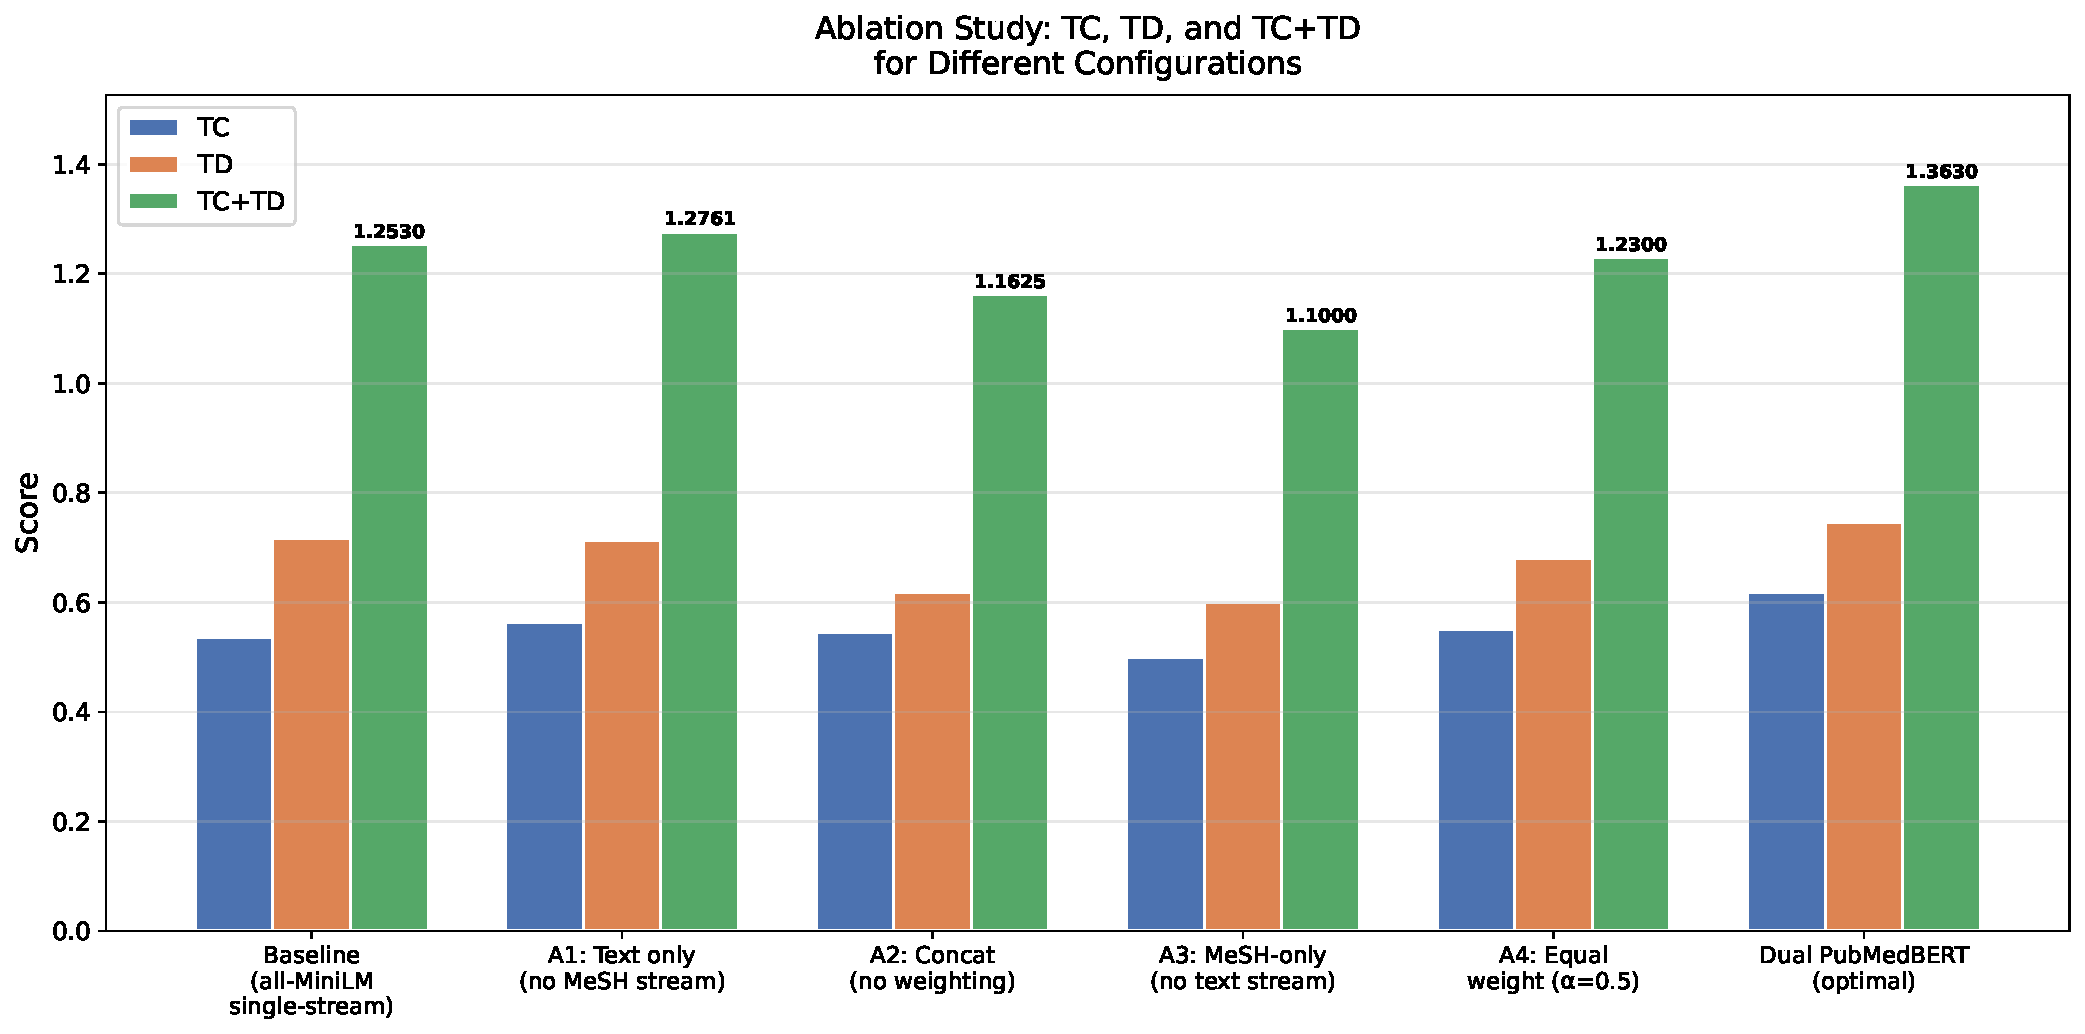
\includegraphics[width=12cm]{./fig/fig_ablation_comparison.pdf}
\caption{Ablation study results showing the progressive performance variation across different input configurations (A1-A4) without parameterized fusion, compared to the baseline and the full dual-stream system with fusion. The Dual-Stream configuration achieves a $3.8\%$ improvement over the baseline (TC+TD: 1.3005 vs. 1.2530). Data source: \textbf{Table~\ref{tab:ablation_results}}.}
\label{fig:ablation}
\end{figure*}

All the experiments used the same random seed and embedding model to ensure strict comparability. A1 replicates the original ``abstract-only'' configuration used in the baseline study. We independently reran this experiment on our own computing infrastructure and obtained results that are extremely close to the reported baseline TC = 0.5428 vs. 0.5360, TD = 0.7136 vs. 0.7170 (see \textbf{Table~\ref{tab:ablation_results}}). The minor discrepancies are likely due to differences in computational environments (e.g., hardware-specific floating-point precision, GPU parallelism effects) rather than methodological inconsistencies.

\textbf{Fig.~\ref{fig:ablation}} demonstrates the impact of different input components on topic modeling performance. The ablation configurations (A1--A4) show inconsistent improvements, with A2, A3, and A4 underperforming the baseline. A closer look at the metric breakdown explains why: across A2--A4, topic coherence (TC) remains roughly stable ($0.527$--$0.545$), whereas topic diversity (TD) deteriorates sharply, from $0.7136$ (A1) to $0.6087$ (A3). The degradation is therefore driven almost entirely by a loss of diversity. This is a direct consequence of naive concatenation: appending MeSH descriptors as plain text injects a small, controlled, and heavily reused vocabulary (e.g., generic descriptors such as \textit{Humans} or \textit{Female}) that the class-based TF-IDF cannot sufficiently down-weight, inflating keyword overlap across topics and collapsing TD; appending titles adds further boilerplate phrasing with the same effect. Because a flat concatenation cannot distinguish a document's core (major) descriptors from incidental (minor) ones, this generic-term noise accumulates rather than being suppressed. The dual-stream design avoids this failure mode by encoding MeSH in a \emph{separate} embedding space and weighting major against minor terms, so that generic descriptors never contaminate the keyword extraction stage. Consequently, the full Dual-Stream configuration with parameterized $\alpha$--$\beta$ fusion achieves TC+TD = 1.3005, a $3.8\%$ improvement over the baseline, confirming that the key innovation lies in the \emph{weighted fusion mechanism} rather than in the inclusion of additional metadata.

Importantly, none of the ablation configurations---despite using the same input components---were able to match the performance of the dual-stream architecture. The proposed full fusion model yielded the highest TC+TD (1.3005), outperforming both the best ablation result (A1, TC+TD = 1.2564) and the baseline (1.2530). This confirms that simply adding information (e.g., full input or MeSH terms) is not sufficient---the performance gains come from structured, weighted integration of unstructured and structured knowledge, not from input volume alone.

\subsection{Effect of the $\beta$ Weighting Scheme}
\label{subsec:beta_norm}

It should be noted that the per-term weighting of $\beta$ (Equation~(\ref{eq:mesh_embedding})) makes the effective document-level contribution of the major-descriptor group depend on the number of major and minor terms in each record. With $M$ major and $m$ minor descriptors, the effective contribution of the major group under the per-term formulation is $M\beta/(M\beta+m(1-\beta))$ rather than $\beta$ itself. In the present corpus, records carry on average substantially more minor than major descriptors (approximately twelve versus two), so the effective major-group contribution is consistently lower than the nominal $\beta$. The parameter $\beta$ therefore acts as a monotonic control that increasingly emphasises major descriptors as it grows, rather than as a literal document-level contribution ratio.

To assess whether this distinction affects topic quality, we compared the per-term formulation with a group-normalised alternative,
\begin{multline}
\boldsymbol{e}_{\text{MeSH}} = \beta\cdot\operatorname{mean}(\{\boldsymbol{e}_i \mid \text{major}\}) \\
+ (1-\beta)\cdot\operatorname{mean}(\{\boldsymbol{e}_j \mid \text{minor}\}),
\label{eq:beta_groupnorm}
\end{multline}
in which the major-to-minor contribution ratio is fixed at $\beta:(1-\beta)$ for every record regardless of term counts (reducing to the mean of whichever group is non-empty when only one type is present). Re-running the optimal Dual PubMedBERT configuration ($\alpha=0.45$) under both formulations at four representative values $\beta \in \{0.20, 0.40, 0.50, 0.60\}$ showed that topic coherence was essentially unchanged (within $0.02$) and that the combined TC+TD score differed only modestly, with neither formulation consistently superior. Topic quality is therefore robust to the precise major/minor weighting scheme. We retain the per-term formulation for consistency with the grid search reported above, while noting that the group-normalised variant in Equation~(\ref{eq:beta_groupnorm}) offers a more direct interpretation of $\beta$ and is preferable for corpora in which the number of MeSH descriptors per record varies widely.

\section{Discussion}

\subsection{Key Findings and Implications}

The experimental results demonstrate the effectiveness of the proposed dual-stream embedding framework for biomedical topic modelling. Three of the four dual-stream configurations outperformed the single-stream baseline on the combined TC+TD metric, with the best configuration---Dual PubMedBERT---achieving TC+TD = 1.3443, a 7.3\% improvement. The one exception, Dual BioBERT, fell 1.6\% below the baseline, indicating that the benefit of dual-stream fusion is conditional on an embedding model whose representation space is well matched to the task: the framework amplifies a suitable encoder rather than compensating for an unsuitable one.

The dual-stream design provides two key benefits. First, it enables semantic complementarity between contextual embeddings, which capture linguistic nuance and discourse structure, and MeSH descriptors, which reflect domain-specific expert annotation. Second, the parameterized weighted fusion mechanism introduces fine-grained control over the contribution of each information type. The grid search showed that moderate $\alpha$ and $\beta$ values yielded the best performance, underscoring the need for balanced integration rather than dominance of either stream.

Crucially, the ablation study confirms that the gains stem from structured integration rather than from additional information alone. All single-stream ablation variants---despite using the same title + abstract + MeSH content---underperformed the dual-stream fusion; the A4 configuration reached only TC+TD = 1.1625, well below the fused counterpart at 1.3005 under the same encoder. Architectural integration, not input volume, is therefore the critical factor. By explicitly encoding and weighting narrative content and curated metadata as separate streams, the framework addresses a limitation of earlier transformer-based methods such as BERTopic, which treat all textual input homogeneously. The LLM-based topic-title generation further improves interpretability, which is particularly valuable for non-expert users such as students and interdisciplinary researchers who require transparent thematic access to biomedical knowledge. The framework's modular embedding, fusion, and topic-modelling stages also make it adaptable to other knowledge-intensive domains without major architectural changes.

\subsection{Comparison with Related Work}
This subsection provides a methodological comparison of our dual-stream embedding framework with existing topic modeling approaches. \textbf{Table~\ref{tab:comparison}} summarizes the key characteristics and design choices of related studies alongside our proposed method.

\begin{table*}[!t]
\centering
\caption{Methodological comparison of the proposed dual-stream framework with representative prior topic-modelling approaches, across method type, embedding representation, MeSH integration, application domain, and key innovation.}
\label{tab:comparison}
\renewcommand{\arraystretch}{1.3}
\begin{tabular}{lclccll}
\hline
\textbf{Reference} & \textbf{Year} & \textbf{Method} & \textbf{Embedding} & \textbf{MeSH} & \textbf{Domain} & \textbf{Key Innovation} \\
\hline
Blei et al.~\cite{blei_latent_2003} & 2003 & LDA & BoW & No & General & Probabilistic topic models \\
Yu et al.~\cite{yu_improving_2016} & 2016 & TopicalMeSH & Word2Vec & Yes & Biomedical & MeSH-based representation \\
Dieng et al.~\cite{dieng_topic_2020} & 2020 & ETM & Word2Vec & No & General & Embedding topic models \\
Angelov~\cite{angelov_top2vec_2020} & 2020 & Top2Vec & Doc2Vec & No & General & Joint doc-topic embeddings \\
Grootendorst~\cite{grootendorst_bertopic_2022} & 2022 & BERTopic & SBERT & No & General & Transformer-based clustering \\
Wang et al.~\cite{wang_graph-embedded_2022} & 2022 & GraphTM & GNN & No & Biomedical & Graph neural networks \\
Lezhnina~\cite{lezhnina_depression_2023} & 2023 & BERTopic & MiniLM & No & Biomedical & Biomedical topic analysis \\
\hline
\textbf{Proposed} & \textbf{2025} & \textbf{Dual-Stream} & \textbf{PubMedBERT} & \textbf{Yes} & \textbf{Biomedical} & \textbf{Parameterized fusion} \\
\hline
\multicolumn{7}{l}{\footnotesize MeSH = Medical Subject Headings integration. BoW = Bag of Words. Bold indicates the proposed method.} \\
\end{tabular}
\end{table*}

As shown in \textbf{Table~\ref{tab:comparison}}, topic modeling methodologies have undergone significant evolution, and our dual-stream framework addresses key limitations of existing approaches through three interconnected innovations.

\textbf{Technical Evolution and Model Selection:} The chronological progression in \textbf{Table~\ref{tab:comparison}} illustrates the advancement from traditional bag-of-words representations (LDA, 2003) through static word embeddings (Word2Vec, Doc2Vec) to contextualized transformer-based encoders (SBERT, PubMedBERT). This evolution reflects the increasing demand for capturing nuanced semantic relationships in text. Our selection of PubMedBERT is motivated by its domain-specific pre-training on biomedical literature, ensuring semantic representations aligned with the specialized vocabulary and conceptual structures inherent to biomedical research.

\textbf{Dual Integration of Domain Knowledge:} Our framework uniquely combines two complementary forms of domain knowledge. First, among all surveyed methods, only Yu et al.'s TopicalMeSH~\cite{yu_improving_2016} and our approach incorporate MeSH terminology; however, TopicalMeSH relies on Word2Vec embeddings that cannot capture contextual semantics. Second, while methods like generic BERTopic~\cite{grootendorst_bertopic_2022} employ general-purpose transformers, our dual-stream design leverages PubMedBERT for domain-specific semantic understanding. This dual integration---structured ontological knowledge (MeSH) with contextualized biomedical representations (PubMedBERT)---addresses both terminological precision and semantic depth, a combination absent in prior work.

\textbf{Parameterized Fusion Mechanism:} The weighted fusion mechanism controlled by parameters $\alpha$ and $\beta$ distinguishes our approach by enabling fine-grained optimization of embedding contributions. Unlike fixed integration schemes in prior methods, our parameterized fusion allows systematic balancing of topic coherence and diversity based on specific retrieval objectives. As demonstrated in \textbf{Table~\ref{tab:model_performance}}, this configurability yields a $7.3\%$ improvement in combined topic quality over the baseline, validating the practical value of adaptive embedding fusion in biomedical topic modeling.

\subsection{Limitations and Future Work}

Despite these encouraging results, this study has several limitations that point toward promising directions for future work.

First, the experiments were conducted on a single, relatively small dataset of 3{,}000 PubMed abstracts, selected to match the conditions of the reference baseline study. While this design enables a clean and controlled benchmark, it has three consequences for the strength of our conclusions. (i)~\textit{Generalizability}: a single thematic corpus may not represent the full heterogeneity of biomedical literature, so the specific optimal $\alpha$--$\beta$ values reported here should be regarded as dataset-dependent rather than universal. (ii)~\textit{External validation}: because all results are obtained on one corpus, we cannot yet claim that the observed improvements transfer to independent datasets or other biomedical subdomains; external validation on separate corpora is needed before the framework is adopted in production retrieval systems. (iii)~\textit{Overfitting risk}: the $\alpha$ and $\beta$ parameters were selected by grid search on the same corpus on which they are evaluated, which may optimistically bias the reported optima. Reassuringly, the high-performing configurations form a broad, contiguous region of the $\alpha$--$\beta$ grid ($\alpha \in [0.15, 0.45]$, $\beta \in [0.15, 0.80]$) rather than isolated spikes, which suggests the effect is robust rather than the product of a single overfitted cell; nevertheless, a held-out tuning/evaluation split would provide a stronger guarantee. Future research should therefore evaluate the scalability and robustness of the framework on larger and more diverse biomedical corpora---including documents that lack MeSH annotations, for which automatic MeSH tagging or prompt-based LLM generation could be explored---and adopt a train/validation/test protocol for parameter selection. The framework is expected to scale gracefully, since, as noted in Section~4, document embeddings are computed once and the fusion adds only an $\mathcal{O}(d)$ operation per document.

Second, the $\alpha$ and $\beta$ parameters were tuned manually via grid search. Although this revealed interpretable and high-performing configurations, it introduces manual overhead and limits adaptability. As part of future development, we aim to implement an automated gating mechanism that dynamically adjusts the fusion weights from document features or a downstream optimization objective, improving usability and generalizability in real-world biomedical information retrieval scenarios.

Third, as discussed in Section~3, the framework currently treats MeSH descriptors as independent terms and does not explicitly exploit the MeSH knowledge organization system---its tree hierarchy, subheading qualifiers, and synonym (entry-term) mappings. These structures encode expert knowledge that a simple weighted average cannot capture: hierarchically close descriptors could be smoothed toward shared ancestors, qualifiers could disambiguate a descriptor's contextual role, and synonym mappings could consolidate lexical variants. Incorporating such information---through hierarchy-aware aggregation, graph-based encoders over the MeSH tree, or qualifier-conditioned embeddings---is a promising avenue for enriching the structured stream and is an important direction for future work.

Such advancements would facilitate integration into interactive biomedical literature retrieval systems, enabling practical deployment in clinical knowledge services, academic libraries, and research support platforms.

\section{Conclusions}

This study demonstrates that the proposed dual-stream embedding framework significantly enhances biomedical topic modeling by synergistically integrating unstructured textual data with structured metadata. Through systematic experimentation and rigorous ablation analysis, we confirmed that the observed improvements in topic coherence and diversity are not merely attributable to increased input information but stem from the architecture's structured, parameterized fusion of semantic and domain-specific knowledge. The fusion parameters ($\alpha$ and $\beta$) allow fine-grained control over the contribution of each stream, and optimal values consistently yield higher-quality topics across multiple evaluation metrics.

Notably, the dual PubMedBERT configuration achieved the highest combined topic quality (TC+TD = 1.3443), surpassing all baseline and ablation models. Even when the same input components (Title, Abstract, MeSH) are used, single-stream models without fusion underperformed, reinforcing the necessity of structured integration. Furthermore, the incorporation of a large language model for post hoc topic labelling significantly improved interpretability, transforming keyword lists into intuitive, academic-style topic summaries suitable for downstream analysis.

Beyond its technical contributions, the framework is scalable, adaptable to other domains, and readily deployable in real-world retrieval systems such as semantic search engines, thematic dashboards, and intelligent literature exploration tools. All source code, processed datasets, and experimental configurations are openly available, enabling full reproducibility and supporting future extensions by the research community. These attributes position the framework as a robust and generalizable foundation for large-scale, user-centered knowledge discovery systems across disciplines.

\acknowledgments
The authors would like to acknowledge the use of the AI language model ChatGPT for assistance in improving the clarity and fluency of the manuscript's English writing. All intellectual content, analyses, and interpretations presented in this work remain solely those of the authors. The use of AI tools complied with the journal's policies on AI-assisted writing.

\bibliographystyle{fujipressbib}
\bibliography{tm-ref}

\acknowledgments[Data Availability]
The dataset used in this study was obtained from the publicly accessible PubMed database. The processed dataset and code supporting the findings of this study are available from the corresponding author upon reasonable request. All code, processed datasets, and experimental results supporting the findings of this study are publicly available at \url{https://github.com/taotao3614/Topic-Modeling-via-a-Dual-Stream-Embedding-Framework}.

\acknowledgments[Conflicts of Interest]
The authors declare that they have no competing interests.

\acknowledgments[Funding]
This research received no specific grant from any funding agency in the public, commercial, or not-for-profit sectors.

\acknowledgments[Ethics Approval]
Not applicable. This study does not involve human participants, human data, or human tissue.

\begin{profile}
	\Name{Tao Tao}
	\Orcid{0009-0005-5277-0001}
	\Affiliation{Graduate School of Science and Technology, Sophia University}
	\Address{Tokyo 102-8554, Japan}
	\History{received the Bachelor of Science degree in food technology and nutrition from the Royal Melbourne Institute of Technology, Melbourne, Australia, in 2018, and the Master of Commerce degree in information systems and technology from Curtin University, Perth, Australia, in 2021. He is currently pursuing the Ph.D. degree in green science and engineering with the Graduate School of Science and Technology, Sophia University, Tokyo, Japan.}
	\Works{$\bullet$ Topic modeling, natural language processing, biomedical informatics, and machine learning}
	\Membership{}
	\Photo{./fig/Tao Tao2024up.jpg}
\end{profile}

\begin{profile}
	\Name{Amena Mahmoud}
	\Orcid{0000-0001-5415-2972}
	\Affiliation{Department of Computer Science, Faculty of Computers and Information, Kafrelsheikh University}
	\Address{Kafrelsheikh 33516, Egypt}
	\History{received the master's degree in computer science from Helwan University, Egypt, in the virtual reality specialization, and the Ph.D. degree in computer science from Mansoura University, Egypt, in the bioinformatics specialization. She is currently an Associate Professor with the Department of Computer Science, Faculty of Computers and Information, Kafrelsheikh University, Egypt, and a Visiting Associate Professor with Sophia University, Japan.}
	\Works{$\bullet$ Bioinformatics, machine learning, pattern recognition, image processing, and natural language processing}
	\Membership{}
	\Photo{./fig/Amena Mahmoud.jpg}
\end{profile}

\begin{profile}
	\Name{Eiko Takaoka}
	\Orcid{0009-0009-2199-8803}
	\Affiliation{Department of Information and Communication Sciences, Faculty of Science and Technology, Sophia University}
	\Address{Tokyo 102-8554, Japan}
	\History{received the Ph.D. degree in engineering from Keio University, Japan, in 1996. She is currently a Professor with the Department of Information and Communication Sciences, Faculty of Science and Technology, Sophia University, Tokyo, Japan, and a Visiting Professor with the Open University of Japan. She is an Associate Member of Science Council of Japan and a Fellow of Information Processing Society of Japan.}
	\Works{$\bullet$ Medical informatics, information education, natural language processing, and database}
	\Membership{$\bullet$ Associate Member of Science Council of Japan; Fellow of Information Processing Society of Japan}
	\Photo{./fig/EikoTakaoka2024up.jpg}
\end{profile}


\end{document}
